\documentclass[12pt]{report}
% Definiciones basicas de LaTeX para la memoria
%
% No modificar las lineas a continuacion a menos
% de estar muy seguro de lo que se esta haciendo!!
%
% Jaime Cisternas, julio 2004, agosto 2010

% <jcisternas@uandes.cl> 

%%%%%%%%%%%%%%%%%%%%%%%%%%%%%%%%%%%%%%%%%%%%%%%%%%%%%%%%%%%%%%%%%%%%%
% Libreria computin
%\usepackage{algorithm}
%\usepackage{algorithmic}
\usepackage[left=3cm,top=2.5cm,right=3cm,bottom=2.5cm]{geometry}

% Encoding

%\usepackage[utf8]{inputenc} % unnecessary when compiling through xelatex
\usepackage[T1]{fontenc}

% Carga librerias utiles con simbolos y estructuras
\usepackage{amsfonts}
\usepackage{amssymb}
\usepackage{amsmath}   
\usepackage{amsthm}
\usepackage{latexsym}
\usepackage{cancel}
\usepackage{physics}
\usepackage{bbm}
\usepackage{listings}
\usepackage{pgfplots}
\usepackage{eurosym}

% Logo Julia

%\usepackage{core/julialogo}

% Cool code highlight
% https://es.overleaf.com/learn/latex/Code_Highlighting_with_minted
% No need of outputdir out of overleaf
\usepackage[outputdir=docs/DocumentoMemoria]{minted}

% Librerías adicionales para diagramas tikz

\usepackage{tikz}
\usepackage{mathdots}
\usepackage{yhmath}
\usepackage{color}
\usepackage{xcolor}
\usepackage{siunitx}
\usepackage{multirow}
\usepackage{gensymb}
\usepackage{tabularx}
\usepackage{extarrows}
\usepackage{booktabs}
\usetikzlibrary{fadings}
\usetikzlibrary{patterns}
\usetikzlibrary{shadows.blur}
\usetikzlibrary{shapes}


% Libreria para ajustar espaciado entre lineas
\usepackage{setspace}

% Libreria con estilo APA para bibliografia
\usepackage{core/newapa}

% Si usted está utilizando un teclado en español, puede ser útil
% usar los paquetes a continuacion. De otra manera tendrá que generar las
% tildes y la letra ñ de forma especial.
% Estos caracteres no pueden ser utilizados en etiquetas ni tampoco en modo matemático
\usepackage[spanish, activeacute]{babel}
\unaccentedoperators


% Declaraciones especificas de pdfLaTeX
\usepackage[%pdftex, % commented to compile with Xelatex
        colorlinks=false,         % true or false (for final version)
        urlcolor=rltblue,         % \href{...}{...} external (URL)
	    anchorcolor=rltbrightblue,
        filecolor=weben,          % \href*{...} local file
        linkcolor=webred,         % \ref{...} and \pageref{...}
        menucolor=webdarkblue,
        citecolor=webgreen,
        pdftitle={},              % INSERT YOUR TITLE HERE
        pdfauthor={},             % INSERT YOUR NAME HERE
        pdfsubject={},
        pdfkeywords={},
        %pdfpagemode=None,
        bookmarksopen=true,
	plainpages=false]{hyperref}
%\usepackage[pdftex]{graphicx}

\usepackage{graphicx}

\usepackage{fontspec}
 
\setmainfont{Times New Roman}



%\pdfcompresslevel=9 %commented to use Xelatex
%\pdfadjustspacing=1 %commented to use xelatex
% Definicion de colores
\usepackage{color}
\definecolor{rltbrightred}{rgb}{1,0,0}
\definecolor{rltred}{rgb}{0.75,0,0}
\definecolor{rltdarkred}{rgb}{0.5,0,0}
\definecolor{rltbrightgreen}{rgb}{0,0.75,0}
\definecolor{rltgreen}{rgb}{0,0.5,0}
\definecolor{rltdarkgreen}{rgb}{0,0,0.25}
\definecolor{rltbrightblue}{rgb}{0,0,1}
\definecolor{rltblue}{rgb}{0,0,0.75}
\definecolor{rltdarkblue}{rgb}{0,0,0.5}
\definecolor{webred}{rgb}{0.5,.25,0}
\definecolor{webblue}{rgb}{0,0,0.75}
\definecolor{webgreen}{rgb}{0,0.5,0}
\definecolor{webdarkblue}{rgb}{0,0,0.5}
\definecolor{webbrightgreen}{rgb}{0,0.75,0}
% fin de declaraciones especificas pdfLaTeX

% tamanio de pagina
%\setlength{\oddsidemargin}{.5in}
%\setlength{\evensidemargin}{.0in} % en caso de usar opcion 'twoside'
%\setlength{\textwidth}{6in}
%\setlength{\topmargin}{-.5in}
%\setlength{\textheight}{9in}


% Las siguientes definiciones pueden ser usadas en
% memorias mas matematicas
\newtheorem{theorem}{Teorema}[section]
\newtheorem{lemma}[theorem]{Lema}
\newtheorem{corollary}[theorem]{Corolario}
\newtheorem{proposition}[theorem]{Proposición}
\newtheorem{definition}[theorem]{Definición}
\newtheorem{claim}{Afirmación}
\newtheorem{conjecture}[theorem]{Conjetura}
\newtheorem{observation}[theorem]{Observación}
\newtheorem{problem}[theorem]{Problema}

% Definicion de un ambiente para algoritmos en pseudo-codigo.
% Esta definicion puede ser mejorada.
\newtheorem{algorithm}{Algoritmo}[section]
\newcommand{\tab}{\hspace*{0.5 cm}}
% Palablas claves que deben aparecer en negrita
\newcommand{\bfWHILE}{\textbf{while~}}
\newcommand{\bfDO}{\textbf{do~}}
\newcommand{\bfEND}{\textbf{end~}}
\newcommand{\bfIF}{\textbf{if~}}
\newcommand{\bfTHEN}{\textbf{then~}}
\newcommand{\bfELSE}{\textbf{else~}}
\newcommand{\bfFOR}{\textbf{for~}}

% Nombres fijos de Latex pueden ser cambiados al Espaniol
\renewcommand{\contentsname}{Índice General}
\renewcommand{\chaptername}{Capítulo}
\renewcommand{\appendixname}{Anexo}
\renewcommand{\bibname}{Bibliografía}
\renewcommand{\figurename}{Ilustración}
\renewcommand{\tablename}{Tabla}
\renewcommand{\indexname}{Índice}
\renewcommand{\partname}{Parte}
\renewcommand{\listfigurename}{Lista de Ilustraciones}
\renewcommand{\listtablename}{Lista de Tablas}

% Para las enumeraciones usamos primero a,b,c,... y despues i, ii, iii,...
\renewcommand{\labelenumi}{\alph{enumi})}
\renewcommand{\labelenumii}{\roman{enumii})}
\renewcommand{\labelenumiii}{-}
\renewcommand{\labelenumiv}{-}

% Para ser consistentes en el uso de abreviaciones!
%\newcommand{\Chp}{Cap\'{\i}tulo}
%\newcommand{\Chps}{Cap\'{\i}tulos}
%\newcommand{\Sec}{Sec.} % \S
%\newcommand{\Secs}{Secs.} % \S\S
%\newcommand{\SSec}{Subsec.}
%\newcommand{\Fig}{Fig.}
%\newcommand{\Figs}{Figs.}
%\newcommand{\Eqn}{Ecn.}
%\newcommand{\Eqns}{Ecns.}

% Muestra en pantalla los nombres de los archivos usados
\listfiles

% Previene una cierta senial de ``warning: contentsline with no destination''
\newcounter{dummy}



\setlength{\parindent}{0cm}
\usepackage{float}
\usepackage{subfigure}
\usepackage{array}
\newcolumntype{E}{>{$}c<{$}}
\usepackage{longtable}
\setcounter{MaxMatrixCols}{40}
\usepackage{bm}


%%%%%%%%%%%%%%%%%%%%%%%%%%%%%%%%%%%%%%%%%%%%%%%%%%%%%%%%%%
\newcommand{\nombreautor}{Eduardo Caballero}
\newcommand{\mes}{Diciembre}
\newcommand{\anio}{2026}
\newcommand{\titulo}{Modelos de redes de crédito bajo información asimétrica}
\newcommand{\nombreprofuno}{Sebastián Cea}
\newcommand{\nombreprofdos}{Claudio Telha}
\newcommand{\nombreproftres}{Nombre Profesor Invitado}
\newcommand{\codigo}{ING-IN-001/11}

%%%%%%%%%%Aqui se escribe el resumen%%%%%%%%%%%%%%%%%%%%%
\newcommand{\resumen}{
Este trabajo evalúa si el modelo de redes financieras duales de Venegas, que extiende el marco de negociación bilateral de Jalan, Chakrabarti y Sarkar, puede calibrarse con datos reales. Dicho modelo predice que una infraestructura alternativa recupera por completo el bienestar que destruye una restricción regulatoria de acceso, aunque lo obtiene con primitivos estipulados. Como caso de aplicación se estudia el programa Crédito Corfo Mipyme, cuyo panel se reconstruye documento a documento desde fuentes públicas, y se audita la implementación numérica heredada. Un ejercicio propio muestra que el hallazgo central descansa casi por completo en una sola entrada de la matriz de covarianzas, la covarianza entre los dos agentes que la restricción separa, ya que la pérdida de bienestar cae de 50,8~\% a 2,4~\% cuando dicha entrada se anula. El diagnóstico muestra que el obstáculo no es de volumen sino de topología, puesto que la red del programa es bipartita y determina precisamente esa entrada, mientras deja sin identificar las varianzas propias y las covarianzas sobre las aristas observadas. El trabajo especifica qué información cerraría la identificación y qué registros se solicitaron a CORFO, de modo que el contraste con la red observada queda condicionado a esa entrega.
}

\newcommand{\agradecimientos}{
Muchas gracias a todos}

\newcommand{\dedicatoria}{\it
ok..
}
\renewcommand{\baselinestretch}{1.5}

%%%%%%%%%%%%%%%%%%%%%%%%%%%%%%%%%%%%%%%%%%%%%%%%%%%%%%%%%%

% Por favor coloque todas las definiciones de simbolos a continuacion
% y no en los archivos de capitulos. Esto evitara la  existencia de
% multiples definiciones para las mismas palabras.

\newcommand{\mydef}
	{\stackrel{\mathrm{def}}{=}}
\newcommand{\e}
	{\hbox{\large{e}}}
\newcommand{\mi}
	{\hbox{\large{i}}}
\newcommand{\RR}{\mathbb{R}}

% El paquete babel en español rotula las tablas como «Cuadro» al iniciar el
% documento, lo que sobrescribe el \tablename de core/preambulo.tex y deja el
% rótulo del PDF en desacuerdo con las referencias en prosa, que dicen «Tabla».
% \addto\captionsspanish aplica el cambio después de babel y lo corrige.
\addto\captionsspanish{%
  \renewcommand{\tablename}{Tabla}%
  \renewcommand{\listtablename}{Índice de tablas}%
}

\geometry{margin=2cm}

%%%%%%%%%%%%%%%%%%%%%%%%%%%%%%%%%%%%%%%%%%%%%%%%%%%%%%%%%%

\begin{document}
\label{start}

% Genera las paginas de titulo, copyright, resumen,
% agradecimientos, dedicatoria, indices,...

% No es necesario modificar

\begin{titlepage}
\tikzset{every picture/.style={line width=0.75pt}} %set default line width to 0.75pt        

\begin{tikzpicture}[x=0.75pt,y=0.75pt,yscale=-1,xscale=1]
%uncomment if require: \path (0,869); %set diagram left start at 0, and has height of 869

%Straight Lines [id:da23590902694809812] 
\draw     (130,0) -- (130,900) ;
%Straight Lines [id:da6870198378646561] 
\draw  [line width=3]   (125,0) -- (125,900) ;
%Straight Lines [id:da620103730055265] 
\draw    (120,0) -- (120,900) ;
%Straight Lines [id:da9595418699780931] 
\draw [line width=3]    (0,150) -- (660,150) ;
%Straight Lines [id:da038904426968975336] 
\draw    (0,155) -- (660,155) ;
%Straight Lines [id:da3582574940086456] 
\draw    (0,145) -- (660,145) ;
%Image [id:dp2636455806851956] 
\draw (62,71.84) node  {
\includegraphics[width=60pt,height=80.96pt]{logos/Logo-UANDES.png}};

% Text Node
\draw (260,37) node [anchor=north west][inner sep=0.75pt]  [font=\normalsize] [align=left] {\begin{minipage}[lt]{179.57pt}\setlength\topsep{0pt}
\begin{center}
UNIVERSIDAD DE LOS ANDES\\FACULTAD DE INGENIERÍA Y\\CIENCIAS APLICADAS
\end{center}

\end{minipage}};
% Text Node
\draw (260,241.86) node [anchor=north west][inner sep=0.75pt]  [font=\LARGE] [align=left] {\begin{minipage}[lt]{206.76pt}\setlength\topsep{0pt}
\begin{center}
\titulo
\end{center}

\end{minipage}};

% Text Node
\draw (260,431) node [anchor=north west][inner sep=0.75pt] [font=\large]  [align=left] {\begin{minipage}[lt]{206.76pt}\setlength\topsep{0pt}
\begin{center}
\nombreautor
\end{center}

\end{minipage}};
% Text Node
\draw (260,495) node [anchor=north west][inner sep=0.75pt]   [align=left] {\begin{minipage}[lt]{206.76pt}\setlength\topsep{0pt}
\begin{center}
TRABAJO PARA OPTAR AL TITULO\\ DE INGENIERO CIVIL INDUSTRIAL
\end{center}

\end{minipage}};
% Text Node
\draw (260,598) node [anchor=north west][inner sep=0.75pt]   [align=left] {\begin{minipage}[lt]{206.76pt}\setlength\topsep{0pt}
\begin{center}
PROFESOR GUÍA: {\sc \nombreprofuno}
\end{center}

\end{minipage}};
% Text Node
\draw (260,681) node [anchor=north west][inner sep=0.75pt]   [align=left] {
\begin{minipage}[lt]{206.76pt}\setlength\topsep{0pt}
\begin{center}
{\small SANTIAGO, DICIEMBRE DE \the\year{}}
\end{center}
\end{minipage}};

% Text Node
\draw (260,755) node [anchor=north west][inner sep=0.75pt]  [font=\normalsize] [align=left] {\begin{minipage}[lt]{206.76pt}\setlength\topsep{0pt}
\begin{center}
UNIVERSIDAD DE LOS ANDES\\FACULTAD DE INGENIERÍA Y\\CIENCIAS APLICADAS
\end{center}

\end{minipage}};

\end{tikzpicture}

\end{titlepage}


%%%%%%%%%%%%%%%%%%%%%%%%%%%%%%%%%%%%%%%%%%

% Escribe la segunda pagina de titulo para ser firmada por la comision

\cleardoublepage
\thispagestyle{empty}

\begin{center}

\vspace*{2cm}
\parbox{10cm}{
\noindent
Certifico que he leído esta memoria y que en mi opinión
su alcance y calidad son completamente adecuados como para ser considerada
una memoria conducente al título de Ingeniero.
\vspace{1cm}

\hfill
\begin{tabular}{c}
\hspace{8cm} \\
\hline
\nombreprofuno \\
(Profesor Guía)
\end{tabular}

\vspace*{1.5cm}

}

\end{center}

%%%%%%%%%%%%%%%%%%%%%%%%%%%%%%%%%%%%%%%%%%

% Espaciado entre lineas
  \onehalfspacing
  %\doublespacing

% Hace pagina de derechos de autor

  \cleardoublepage
  \thispagestyle{empty}
  %\vspace*{0in}
  \begin{center}
    \copyright\ \nombreautor\ \the\year{} \\
    Todos los derechos reservados.
  \end{center}

%%%%%%%%%%%%%%%%%%%%%%%%%%%%%%%%%%%%%%%%%%%%%%%%%%%%%%%%%%%%%%%%%%%%%%

% Genera agradecimientos leyendo definicion de agradecimientos
\pagenumbering{roman}
  \cleardoublepage \addcontentsline{toc}{section}{Agradecimientos}
  \begin{center} \Large \textbf{Agradecimientos} \end{center}


% Genera resumen leyendo definicion de resumen


  \cleardoublepage
  \refstepcounter{dummy} \addcontentsline{toc}{section}{Resumen}
  \begin{center} \Large \textbf{Resumen} \end{center}
\resumen



% Genera dedicatoria

 % \cleardoublepage \vspace*{1.5in}
  %\begin{flushright} \dedicatoria %\end{flushright}

% Produce indice general, listas de figuras y de tablas

  \cleardoublepage
  \tableofcontents
  \cleardoublepage
  \listoffigures
  \cleardoublepage
  \listoftables
  \cleardoublepage

  \normalsize
  \pagenumbering{arabic}

%%%%%%%%%%%%%%%%%%%%%%%%%%%%%%%%%%%%%%%%%%%%%%%%%%%%%%%%%%%


%%%%%%%%%%%%%%%%Ingreso de capitulos%%%%%%%%%%%%%%%%%%%%%%

% cap1.tex

\chapter{Introducción}
\label{c1} % la etiqueta para referencias

% ============================================================
% Contenido retomado de Proyecto de Título I (PT1), Hito 1 (Hito_1.tex)
% ============================================================

Las infraestructuras financieras alternativas al sistema bancario tradicional, agrupadas bajo el concepto de \textit{shadow banking} o \textit{non-bank financial intermediation} (NBFI), representan hoy USD~238 billones a nivel global, equivalentes
al 49,1\% de los activos financieros mundiales \cite{fsb_global_2024}. Esta escala
convierte en un problema económico relevante el estudio de cómo las restricciones
regulatorias sobre las redes financieras tradicionales inciden en el bienestar
agregado. En consecuencia, cobra relevancia investigar bajo qué condiciones la coexistencia de infraestructuras con
regulaciones distintas (tradicionales y alternativas como por ejemplo \textit{blockchain}) puede recuperar parte o la totalidad de ese bienestar.

El presente trabajo se enmarca en la extensión del modelo de redes financieras duales
propuesto por \citeA{venegas_reyes_financial_2025}, quien a su vez extiende el marco
de negociación bilateral en redes de \citeA{jalan_incentive-aware_2024}. El modelo
de \citeA{venegas_reyes_financial_2025} muestra que, cuando una restricción regulatoria impide el
contrato directo entre dos agentes, la sola competencia entre intermediarios
habilitados recupera solo parcialmente el bienestar perdido. Habilitar
una infraestructura alternativa con regulación distinta, donde el contrato prohibido en la red tradicional sí puede ejecutarse, logra una recuperación completa del bienestar agregado. Este resultado, sin embargo, se obtiene bajo parámetros ilustrativos y no calibrados contra datos reales, lo que limita su interpretación cuantitativa y su valor como evidencia para política regulatoria.

En función de lo anterior se establece el siguiente objetivo general.

\section{Objetivos}
\label{c1:objetivos}

Se busca evaluar la capacidad del modelo de redes financieras duales de \citeA{venegas_reyes_financial_2025} para representar y predecir la recuperación de bienestar observada en un caso con datos reales.  Ese ejercicio genera un insumo de validación empírica que la tesis de \citeA{venegas_reyes_financial_2025} no desarrolla y que resulta valioso para una eventual publicación relacionada en una revista de finanzas o de investigación de operaciones.

\subsection{Objetivo general}

Aplicar un modelo de redes financieras a datos reales para evaluar cambios en bienestar. El objetivo general se lleva a cabo a través de los siguientes objetivos específicos.

\subsection{Objetivos específicos}

\begin{enumerate}
    \item Evaluar la factibilidad de calibrar los primitivos del modelo de \citeA{venegas_reyes_financial_2025}, por ejemplo, creencias de retorno, matrices de covarianza y coeficientes de aversión al riesgo.
    \item Implementar y validar numéricamente el modelo base contra los \textit{benchmarks} ya desarrollados por \citeA{venegas_reyes_financial_2025}.
    \item Aplicar el modelo calibrado al caso de datos reales seleccionado y contrastar sus predicciones de bienestar y de reparto de actividad entre redes con la evidencia observada.
\end{enumerate}

\section{Preguntas de investigación}
\label{c1:preguntas}

Con base en el marco de \citeA{venegas_reyes_financial_2025} y bajo el enfoque
empírico descrito en el Capítulo~\ref{c3}, este trabajo busca responder tres
preguntas que el modelo original, calibrado solo con parámetros ilustrativos, no
puede responder por sí mismo.

\begin{enumerate}
    \item ?`Persiste la recuperación (parcial o completa) del bienestar que predice
    el modelo de \citeA{venegas_reyes_financial_2025} cuando sus parámetros se
    calibran con datos reales,
    en lugar de valores ilustrativos?
    \item ?`Es consistente el reparto de actividad entre la red tradicional y la
    red alternativa que predice el modelo con el reparto efectivamente observado
    en el caso de datos reales seleccionado?
    \item ?`Cómo se distribuyen, en el caso calibrado, las ganancias de bienestar
    entre los agentes de la red, y coincide esa distribución con la que predice el
    modelo teórico?
\end{enumerate}

Las tres preguntas se formulan sobre la versión homogénea del modelo, con foco
en su validación empírica, según el alcance que delimita la sección siguiente.

\section{Alcances}
\label{c1:alcances}

El trabajo se circunscribe a la validación empírica del modelo de redes duales
de \citeA{venegas_reyes_financial_2025} en su versión homogénea, es decir, con
$\gamma_i = 1$ para todo agente y creencias comunes. Dentro de ese marco se
abordan la selección de un caso real de financiamiento en Chile, el
levantamiento de las series públicas que describen sus flujos, la declaración de
los supuestos necesarios para las variables que ninguna fuente observa, la
calibración de los primitivos del modelo y el contraste de sus predicciones con
la evidencia disponible.

Quedan fuera del alcance tres líneas de trabajo. La primera es la extensión del
modelo a agentes heterogéneos en aversión al riesgo y creencias, que exige un
desarrollo analítico propio y se deja como trabajo futuro. La segunda es la
incorporación de dinámica, dependencia de trayectoria y riesgo de contagio al
modelo dual, identificadas como oportunidades de mejora en la
Sección~\ref{c24:oportunidades} pero ajenas al objetivo de validación. La
tercera es la estimación de aquellas entradas de $\Sigma$ que la estructura de la
red del caso deja sin identificar, esto es, las varianzas propias y las
covarianzas a lo largo de las aristas observadas, las que se reportan como no
identificadas en lugar de estimarse, según se argumenta en la
Sección~\ref{c24:identificacion} y se cuantifica en la
Sección~\ref{c3:identificabilidad}.

\section{Metodología}
\label{c1:metodologia}

El trabajo se desarrolla en cinco etapas. La primera consiste en el estudio del
marco teórico de redes financieras, de la competencia entre infraestructuras y
del modelo dual que este trabajo valida, lo que constituye el contenido del
Capítulo~\ref{c2}. La segunda corresponde a la verificación de la implementación
numérica publicada junto con el modelo que se valida, de modo que una
discrepancia posterior con los datos no pueda atribuirse a ella. La tercera
corresponde a la selección de un caso real cuya topología reproduzca la
estructura de dos redes del modelo y al levantamiento de las fuentes públicas
que describen sus flujos de financiamiento. La cuarta consiste en la prueba de
factibilidad empírica, que confronta los datos efectivamente disponibles con los
requisitos formales de identificación y estimación del marco teórico. La quinta
corresponde a la calibración de los primitivos del modelo, al cálculo del punto
estable y al contraste de las predicciones de bienestar y de reparto de
actividad entre redes con la evidencia observada. Las etapas segunda a quinta se
detallan en el Capítulo~\ref{c3}.

\section{Estructura del documento}
\label{c1:estructura}

El documento se organiza en cinco capítulos. El presente capítulo introduce el
problema, los objetivos, las preguntas de investigación y el alcance del
trabajo. El Capítulo~\ref{c2} reúne el marco teórico, desde los modelos de
referencia de redes financieras hasta el modelo de redes duales y los
resultados formales sobre existencia del equilibrio, convergencia de las
negociaciones bilaterales e identificación de los primitivos a partir de datos.
El Capítulo~\ref{c3} presenta el desarrollo metodológico, que comprende el
estudio del marco de referencia, la verificación de la implementación publicada,
el caso de aplicación, las fuentes de datos levantadas, los supuestos adoptados
para las variables no observadas, el diagnóstico de factibilidad empírica y el
procedimiento de calibración. El Capítulo~\ref{c4} expone el análisis de los resultados
de la calibración y el Capítulo~\ref{c5} recoge las conclusiones y
recomendaciones. Los anexos reúnen el material de referencia, esto es, la
notación del modelo y el detalle de las fuentes de datos consultadas.




% cap2.tex

\chapter{Marco Teórico}
\label{c2}

% ============================================================
% Contenido retomado de Proyecto de Título I (PT1), Hito 1 (Hito_1.tex)
% ============================================================

El presente capítulo reúne el marco teórico que sustenta el análisis de redes
financieras desarrollado en este trabajo. Se revisan en primer lugar los modelos
de referencia de la literatura de redes financieras, a continuación los dos
cuerpos teóricos que explican la competencia entre infraestructuras y la
aparición de infraestructuras alternativas, y finalmente el modelo de redes
duales de \citeA{venegas_reyes_financial_2025} junto con los resultados formales
de \citeA{jalan_incentive-aware_2024} sobre existencia, convergencia e
identificación que la validación empírica del Capítulo~\ref{c3} requiere.

\section{Modelos de redes financieras}\label{c22}

Se definen las redes como conexiones entre nodos y \textit{links}: los agentes
(nodos) toman decisiones estratégicas sobre con quiénes formar vínculos,
considerando los beneficios esperados y sus costos \cite{jackson_strategic_1996}. Con base en estas redes se modelan fenómenos como el contagio financiero, la propagación del riesgo sistémico y la estabilidad del sistema económico. La literatura distingue tres
modelos de referencia:

\begin{itemize}
    \item \textbf{\citeA{eisenberg_systemic_2001}:} representan las redes
    financieras a través de una matriz de obligaciones entre agentes. El modelo se distingue pues captura el efecto
    cascada en la red cuando ocurre un \textit{default}, mostrando la existencia
    y unicidad de un vector de pagos que liquida el sistema.

    \item \textbf{\citeA{elliott_financial_2014}:} modelan el contagio financiero en dos dimensiones. La primera dimensión corresponde a la dependencia de contraparte (integración) y la segunda por el número de contrapartes por agente (diversificación). Se distingue en el modelo que ambas dimensiones tienen efectos no monótonos sobre la amplificación o mitigación del riesgo sistémico.

    \item \textbf{\citeA{jalan_incentive-aware_2024}:} introducen una matriz cuadrada para representar origen-destino junto con otra matriz $Q$, simétrica y semidefinida positiva, que captura la estructura de costos y
    beneficios entre pares de agentes. Además utiliza una función de utilidad media-varianza que permite modelar decisiones óptimas de contratación bilateral en un equilibrio \textit{pairwise stable}. Es el modelo base sobre
    el cual se construye la tesis de \citeA{venegas_reyes_financial_2025}, que este
    trabajo extiende.
\end{itemize}

% TODO (autor): incluir desarrollo posterior a la revision de literatura.

\paragraph{Propagación de riesgo y estabilidad.}

Las redes financieras tradicionales son particularmente vulnerables al contagio
cuando falla un nodo crítico, como un banco sistémico. Como muestran \citeA{glasserman_contagion_2016}, las redes densamente conectadas pueden ser resilientes ante \textit{shocks} pequeños, pero frágiles ante crisis sistémicas. Además demuestran que la conectividad absorbe perturbaciones locales, pero también amplifica los choques de gran magnitud. En la misma línea, \citeA{acemoglu_systemic_2015} documentan que la diversificación de conexiones
incrementa inicialmente la estabilidad del sistema, pero más allá de cierto
umbral la interdependencia generada abre nuevos canales de riesgo sistémico. Es
decir, la relación entre conectividad y estabilidad no es monótona.

Las redes financieras tradicionales presentan, además, limitaciones estructurales
documentadas extensamente en la literatura:

\paragraph{Altos costos de intermediación.}
Los intermediarios financieros tales como bancos o cámaras de compensación imponen comisiones por transferencias internacionales y por gestión de riesgo y cumplimiento regulatorio que en promedio alcanzan un $6,36\%$ del monto enviado a nivel mundial (más del doble de la meta de $3\%$ fijada en el ODS 10.c), cifra que baja a $4,59\%$ cuando la transferencia se realiza por canales digitales frente a $7,30\%$ en canales no digitales \cite{world_bank_rpw_2025}. Esto constituye una barrera a la inclusión financiera, en particular en mercados emergentes.

\paragraph{Opacidad y asimetrías de información.}
La información transaccional suele restringirse a las partes directamente
involucradas, lo que dificulta evaluar el riesgo de una contraparte y favorece
el comportamiento oportunista.

\paragraph{Riesgo sistémico y centralización.}
La centralización en instituciones clave como grandes bancos y mercados
centralizados crea puntos únicos de falla. \citeA{elliott_financial_2014}
señalan que esta concentración del riesgo hace a las redes tradicionales más
susceptibles de propagar shocks macroeconómicos o eventos de liquidez. En
contraste, \citeA{gofman_efficiency_2017} argumentan que los bancos grandes e
interconectados pueden mejorar la eficiencia agregada. Esto, precisamente porque
reducen el largo de las cadenas de intermediación en el mercado. El efecto neto depende de si domina la reducción de fricciones de intermediación o la concentración del riesgo, de modo que la centralización no es unívocamente negativa.

\paragraph{Baja inclusión financiera.}
Las redes tradicionales suelen excluir a agentes que no cumplen criterios
formales de acceso como un historial crediticio, cuenta bancaria. Un problema
particularmente agudo en economías en desarrollo, donde aproximadamente 2 mil millones de adultos (un $38\%$ de la población adulta mundial, cifra de 2014) permanecían fuera del sistema financiero formal \cite{singer_financial_2017}.

\paragraph{Efectos de red.}
Una mayor conectividad amplía el acceso a financiamiento y permite diversificar
riesgo. Por otra parte, también puede generar congestión operacional y mayores costos transaccionales a medida que la red crece \cite{hinzen_bitcoins_2022,iyengar_economics_2023}.

\section{Competencia entre infraestructuras financieras}\label{c23}

La competencia entre redes Tradicional y Alternativa que este trabajo analiza, que \citeA{venegas_reyes_financial_2025} modela formalmente, se apoya en dos
cuerpos de literatura complementarios. El primero, la teoría de plataformas y mercados de
dos lados que explica cómo compiten infraestructuras con efectos de red. Segundo, el arbitraje regulatorio que explica por qué surgen infraestructuras alternativas.

\subsection{Mercados de dos lados y competencia entre plataformas}

\citeA{economides_economics_1996} establece que las redes financieras
funcionan económicamente como plataformas debido a externalidades de red. La
utilidad de una conexión financiera aumenta con la liquidez y profundidad de la
red a la que pertenece. \citeA{rochet_platform_2003} formalizan esta idea en el
marco de mercados de dos lados. Este concepto se define como mercados donde una plataforma
habilita interacciones entre dos grupos de usuarios y donde el valor para un
lado depende críticamente de la participación del otro lado (externalidades de
red \textit{indirectas}). Traducido en el contexto de redes financieras, estos dos lados se pueden entender como oferentes de liquidez (capital disponible para prestar o
invertir) y demandantes de liquidez (agentes que buscan financiamiento o
cobertura).

Por su parte, \citeA{armstrong_competition_2006} extiende este marco a la competencia entre
múltiples plataformas e identifica tres escenarios según el patrón de
participación de los agentes. \textit{single-homing}, los usuarios se afilian a
una sola plataforma, lo que tiende a generar resultados de tipo
\textit{winner-take-all}. \textit{multi-homing}, donde los usuarios se afilian a varias plataformas simultáneamente, lo que suaviza la competencia y permite la coexistencia. Por último, en los \textit{cuellos de botella
competitivos}, un lado se afilia a una sola plataforma mientras el otro se
multi-afilia. El resultado central de Armstrong es que la coexistencia de
infraestructuras es viable cuando el costo de multi-homing es moderado y las
plataformas se diferencian. Ya que, si el costo es muy alto, el mercado tiende a concentrarse en una sola infraestructura.

Este marco aplica directamente al modelo dual de \citeA{venegas_reyes_financial_2025}: la variable de decisión $(w_i^T, w_i^A)$ es, finalmente, una decisión de multi-homing entre la red Tradicional y la Alternativa. El parámetro de
fricción $\lambda_A$ representa el costo de ese multi-homing. \citeA{caillaud_chicken_2003} muestran que la diferenciación entre plataformas actúa como un mecanismo que suaviza la competencia directa. Esta diferenciación puede darse por ejemplo en la transparencia o en el tipo de contratos que cada red permite. De esta forma se sostiene la coexistencia entre plataformas, en lugar de forzar un resultado de dominancia total de una infraestructura sobre la otra.

\subsection{Arbitraje regulatorio}

Un elemento central para entender por qué surgen infraestructuras alternativas es el concepto de \textbf{arbitraje regulatorio}. Se conceptualiza esta dinámica por \citeA{kane_good_1977} como la ``dialética regulatoria''. Quien a su vez la define como un proceso cíclico en que la regulación induce a los agentes económicos a innovar tecnológicamente, con el único fin de eludir restricciones costosas. A diferencia de modelos estáticos donde los agentes aceptan pasivamente las restricciones, el volumen ``excluido'' busca nuevos canales, dando origen a un sistema ``en la sombra''.

Esta dinámica está documentada empíricamente por \citeA{buchak_fintech_2018}, quienes encuentran evidencia causal de que el arbitraje regulatorio es un motor determinante del crecimiento \textit{Fintech}. 
Estiman que cerca del $50\%$ de la expansión del \textit{shadow banking} responde a la carga regulatoria sobre la banca tradicional (mayores requerimientos de capital, entre otros).
Por lo tanto, no se trata solo de una decisión de preferencia por la tecnología que la acompaña.
Esto valida el mecanismo central del modelo dual, que consiste en que la migración de volumen hacia la red Alternativa ($w_i^A$) es una respuesta económica racional a la fricción regulatoria en el sector incumbente, no meramente una preferencia tecnológica.
La literatura, sin embargo, no es unánime sobre las implicancias de bienestar de
este arbitraje. \citeA{buchak_fintech_2018} lo interpretan como una
respuesta eficiente a restricciones costosas. Por su parte, \citeA{gorton_regulating_2010}
advierten que el \textit{shadow banking} puede ser también una fuente de
inestabilidad sistémica, precisamente por operar con menor transparencia y
supervisión que el sistema regulado. El parámetro de transparencia $\tau$ en el
modelo dual puede leerse como una forma de capturar esta tensión. Una infraestructura alternativa transparente ($\tau > 0$) podría ofrecer los beneficios de eficiencia del arbitraje regulatorio, sin heredar necesariamente
los riesgos típicamente asociados al \textit{shadow banking} opaco.

\subsection{Adopción tecnológica, efectos de red y dependencia de trayectoria}

La adopción de una infraestructura financiera alternativa enfrenta, además,
problemas de coordinación característicos de mercados con externalidades de
red. \citeA{katz_network_1985} muestran que las tecnologías con externalidades
de red positivas, donde el valor para cada usuario aumenta con el número de
otros usuarios, enfrentan un problema de coordinación fundamental. Los adoptantes potenciales pueden preferir no adoptar si esperan que pocos otros lo hagan, incluso cuando la adopción universal beneficiaría a todos. 
Esto genera \textit{exceso de inercia}, que consiste en que el mercado permanece anclado a una tecnología
inferior porque los agentes esperan racionalmente que otros sigan usando el
estándar establecido. También causa equilibrios múltiples para los mismos parámetros
fundamentales, dependiendo únicamente de las expectativas sobre el
comportamiento de los demás.

\citeA{farrell_installed_1986} formalizan el concepto de \textit{exceso de
inercia} sobre cómo una tecnología establecida con una base
de usuarios grande puede resistir la competencia de alternativas objetivamente
superiores, porque cada agente racionalmente espera que otros se muevan
primero. La red Tradicional posee, en este sentido, una base ya instalada con relaciones existentes, infraestructura, marcos regulatorios y procedimientos operacionales, base que la red Alternativa debe superar con beneficios de transparencia ($\tau$) suficientemente grandes para compensar tanto los costos de fricción directos ($\lambda_A$) como la ventaja de coordinación de la red incumbente.

\citeA{arthur_competing_1989} extiende esta lógica introduciendo los conceptos
de \textit{path dependence} y \textit{lock-in} en mercados con retornos
crecientes a la adopción. Cuando una tecnología exhibe retroalimentaciones
positivas, pequeños accidentes históricos o ventajas tempranas pueden llevar a
la dominancia permanente de una tecnología, incluso si otra es objetivamente
superior. Aplicado al modelo dual, esto implica que la asignación inicial
$w_i^*$, heredada del equilibrio de red única sin restricciones, condiciona el
punto de partida desde el cual se evalúa la adopción de la red Alternativa. La
multiplicidad de equilibrios del modelo dual (cuando $Z_F^{\text{dual}}$ no
tiene rango completo) puede interpretarse precisamente como una manifestación de
esta dependencia de trayectoria.

\section{Blockchain y finanzas descentralizadas}

La tecnología \textit{blockchain}, introducida por \citeA{nakamoto_bitcoin_2008}
como la estructura subyacente de Bitcoin, es un sistema de registro
distribuido que permite consignar transacciones de forma segura, transparente e
inmutable. Esto se logra a través de una red de nodos, sin requerir una autoridad central que
controle el libro de cuentas. \citeA{cong_blockchain_2019} identifican cuatro
mecanismos económicos centrales a través de los cuales blockchain afecta los
resultados de mercado:

\begin{itemize}
    \item \textbf{Transparencia y auditabilidad}, ya que todas las transacciones quedan registradas en un libro público e inmutable, verificable por cualquier participante.
    \item \textbf{Automatización vía \textit{smart contracts}}, que permite ejecutar términos contractuales sin depender de intermediarios de confianza, reduciendo el riesgo de contraparte.
    \item \textbf{Desintermediación}, al habilitar transacciones directas entre pares.
    \item \textbf{Composabilidad}, que permite construir productos financieros complejos combinando contratos más simples.
\end{itemize}

Estos mismos autores advierten que estas propiedades introducen nuevas disyuntivas entre eficiencia y otros
objetivos, como privacidad o flexibilidad contractual que no están presentes en
las redes tradicionales.

La evidencia empírica sobre blockchain como infraestructura alternativa es
mixta. \citeA{makarov_blockchain_2021}, en un análisis extenso del mercado de
Bitcoin, documentan que la transparencia transaccional reduce ciertas asimetrías
de información. Los participantes sofisticados pueden observar patrones de flujo
y comportamiento de las contrapartes en tiempo real. Simultáneamente crea
nuevas ventajas de información para quienes tienen mayor capacidad analítica
sobre los datos \textit{on-chain}. Además, encuentran que los costos de
transacción son altamente variables y pueden dispararse durante periodos de
congestión de red. \citeA{huberman_monopoly_2021} caracterizan este fenómeno
como un ``monopolio sin monopolista''. El protocolo restringe la oferta de
espacio de bloque, generando precios de monopolio, pero ninguna entidad
individual captura esas rentas (que van, en cambio, a los mineros o validadores).
Esta evidencia empírica sobre costos variables y crecientes con la congestión es
consistente con la forma funcional cuadrática $\lambda_A \|w_i^A\|^2$ que el
modelo dual utiliza para representar el costo de fricción de la red Alternativa.

\citeA{schar_decentralized_2021} identifica los canales concretos a través de
los cuales la transparencia de blockchain crea valor económico. En primer lugar, reduce la
selección adversa en mercados \textit{over-the-counter} al hacer observables
los historiales transaccionales. Además, mejora el monitoreo de riesgo de contraparte.
También habilita la ejecución \textit{trustless} de operaciones complejas sin depender
de intermediarios humanos. Por último, facilita la auditoría regulatoria. Sin embargo,
\citeA{werbach_trust_2018} matiza esta lectura. La evidencia de vulnerabilidades
en \textit{smart contracts}, la persistencia de mecanismos de gobernanza humana
para resolver disputas, y el llamado ``problema del oráculo'' (la necesidad de
información externa confiable para que los contratos inteligentes funcionen)
muestran que blockchain no elimina la confianza. En realidad, la redistribuye de
la confianza en instituciones humanas a la confianza en código, criptografía y
mecanismos de consenso. Sus beneficios dependen del contexto institucional
específico. Estos mecanismos, transparencia con beneficios acotados por
limitaciones prácticas, son los que el parámetro $\tau$ del modelo dual busca
capturar de forma neta.

Finalmente, la diferencia regulatoria entre redes Tradicional y Alternativa
($\Psi_i^T \neq \Psi_i^A$) tiene respaldo institucional directo.
\citeA{zetzsche_decentralized_2020} documentan que los sistemas
descentralizados suelen operar en zonas grises regulatorias. Esto surge por la dificultad
de determinar qué jurisdicción aplica a un protocolo global, lo que habilita cierto arbitraje jurisdiccional pero también genera incertidumbre legal. 
\citeA{auer_rise_2023}, en un estudio del Banco de Pagos Internacionales, documentan un patrón de adopción institucional \textit{bifurcado}. 
Las instituciones financieras grandes y reguladas experimentan principalmente con
\textit{blockchains} permisionados que preservan privacidad y cumplimiento
regulatorio. 
Mientras que entidades más pequeñas o menos reguladas adoptan más directamente sistemas públicos y sin permisos. 
En ambos casos, la adopción se concentra en casos de uso específicos como pagos transfronterizos, financiamiento de comercio o liquidación de valores, en lugar de un reemplazo total de la infraestructura existente. 
Este patrón de adopción parcial y heterogénea entre instituciones es consistente con la predicción del modelo dual de que la
asignación óptima $w_i^{A*}$ es, en general, estrictamente interior
($0 < w_i^{A*} < w_i^*$) y no una migración completa hacia la red Alternativa.

\section{Un modelo de redes duales}
\label{c24}

Esta sección presenta el modelo base de \citeA{jalan_incentive-aware_2024}, la
extensión dual de \citeA{venegas_reyes_financial_2025} y los resultados formales
de ambos marcos que sostienen la aplicación empírica desarrollada en el
Capítulo~\ref{c3}. La notación empleada en el resto del documento se resume en
la Tabla~\ref{tab:notacion} del Anexo~\ref{anexo:notacion}. De los resultados de
\citeA{jalan_incentive-aware_2024} se recogen aquí los que sostienen la
calibración empírica, quedando fuera los de su Sección 3, relativos a
fricciones, estática comparativa y detección de la fuente de un cambio en la
red, por no tener relación directa con ese ejercicio.

El modelo base de \citeA{jalan_incentive-aware_2024} considera una red de $n$
agentes que negocian contratos bilaterales bajo una función de utilidad
media-varianza. Cada agente $i$ posee un vector de creencias $\mu_i$ sobre los
retornos esperados, una matriz de covarianzas $\Sigma_i$ y un coeficiente de
aversión al riesgo $\gamma_i$. La utilidad de un agente $i$ toma la forma
\begin{equation}
\label{eq:utilidad}
    g_i(W, P) = w_i^\top (\mu_i - P e_i) - \gamma_i\, w_i^\top \Sigma_i\, w_i,
\end{equation}
sujeta a una restricción regulatoria capturada por una matriz de proyección
$\Psi_i$. La solución óptima de la Ecuación~\eqref{eq:utilidad} admite la forma
cerrada
\begin{equation}
\label{eq:optimo}
    w_i^* = Q_i(\mu_i - P e_i),
    \qquad
    Q_i = \Psi_i^\top \left( 2\gamma_i\, \Psi_i \Sigma_i \Psi_i^\top \right)^{-1} \Psi_i ,
\end{equation}
donde $Q_i$ es la matriz de sensibilidad del agente $i$. Una asignación $(W,P)$ es
\textit{pairwise stable} si ningún par de agentes puede mejorar simultáneamente
desviándose unilateralmente de ella.

\citeA{venegas_reyes_financial_2025} extiende este marco introduciendo dos
infraestructuras paralelas. Primero, una red Tradicional ($T$) con restricción
regulatoria $\Psi_i^T$. Segundo, una red Alternativa ($A$) con restricción $\Psi_i^A$.
Cada agente reparte su exposición total entre ambas según la partición
\begin{equation}
\label{eq:particion}
    w_i^* = w_i^T + w_i^A ,
\end{equation}
y la utilidad incorpora un beneficio de transparencia $\tau \geq 0$ de la red
alternativa y un costo friccional cuadrático $\lambda_A \geq 0$ sobre $w_i^A$,
\begin{equation}
\label{eq:utilidad-dual}
    g_i(W, P) = w_i^\top (\mu_i + \tau e^A_i - P e_i) - \gamma_i\, w_i^\top \Sigma_i\, w_i
    - \lambda_A \|w^A_i\|^2 .
\end{equation}
El modelo dual es consistente con el modelo base de Jalan y Chakrabarti en tres
casos límite. Cuando $\lambda_A \to 0$ y $\tau = 0$, cuando $\Psi^A$ desactiva
todos los contratos y finalmente cuando $\Psi^T = \Psi^A$.

\subsection{Factibilidad y estabilidad de una asignación}
\label{c24:estabilidad}

Las Definiciones 2 y 3 de \citeA{jalan_incentive-aware_2024} precisan qué
significa formalmente un punto de equilibrio de la red. Una tupla $(W,P)$ es
factible si $W=W^\top$, $P=-P^\top$, y ambas obedecen las restricciones de red
codificadas en $(\Psi_i)_{i\in[n]}$. Es estable si, además, cada agente $i$
maximiza su utilidad $g_i(W,P)$ dado $P$, sobre todas las alternativas factibles
$W'$ que solo modifican su propia fila y columna. En consecuencia, $(W,P)$ es
estable cuando ningún agente puede mejorar unilateralmente su utilidad
renegociando sus contratos vigentes, que es el sentido en que se interpreta el
equilibrio de la red del caso de aplicación del Capítulo~\ref{c3}.

\subsection{Existencia y unicidad del punto estable}
\label{c24:teorema1}

Bajo condiciones generales, el Teorema 1 de \citeA{jalan_incentive-aware_2024}
establece que el punto estable es único y se obtiene resolviendo el sistema
lineal
\begin{equation}
\label{eq:teorema1}
    Z_F \cdot \mathrm{uvec}(P)_F = \mathrm{uvec}(A-A^\top)_F ,
\end{equation}
donde $F$ es el conjunto de aristas permitidas y $Z_F$ se construye a partir de
las matrices de sensibilidad $Q_i$ definidas en la Ecuación~\eqref{eq:optimo}.
% TODO (autor): explicitar la definicion de la matriz A segun Jalan y Chakrabarti (2024).
La Ecuación~\eqref{eq:teorema1} es el mecanismo que, dado un conjunto de
creencias $(M,\Gamma,\Sigma)$, entrega el tamaño de contrato predicho por el
modelo para cada par de agentes, y es por lo tanto el resultado que articula la
calibración empírica desarrollada en el Capítulo~\ref{c3}.

\subsection{Negociaciones bilaterales y convergencia}
\label{c24:algoritmo1}

En la práctica, el punto estable se alcanza mediante negociaciones bilaterales
iterativas (Algoritmo 1 de \citeA{jalan_incentive-aware_2024}), en las que, en
cada ronda, todos los pares de agentes permitidos actualizan simultáneamente su
precio $P_{ij}$ hacia el valor que resuelve su desacuerdo, ponderado por un
factor de amortiguación $\eta \in (0,1)$. El Teorema 4 establece que la
convergencia está garantizada para
\begin{equation}
\label{eq:eta}
    \eta < \eta^* = \frac{2}{\lambda_{\max}} ,
\end{equation}
donde $\lambda_{\max}$ es el autovalor máximo de la matriz $(L^\dagger K)|_R$
construida a partir de las mismas matrices $Q_i$. El interés de este mecanismo
descentralizado es que cada par negocia usando solo su propio precio vigente,
sin necesidad de conocer de antemano toda la red, tal como lo haría un agente
real.

\subsection{Resultado central}
\label{c24:resultado}

Sobre una red de tres agentes, Banco Nacional ($N$), Banco Local ($L$) y Empresa
Local ($F$), donde la regulación prohíbe el contrato directo $N$--$F$,
\citeA{venegas_reyes_financial_2025} muestra que la sola competencia entre
intermediarios habilitados (incorporando una cuarta firma que compite con $L$)
recupera solo parcialmente el bienestar perdido por la restricción. Esta deja un
\textit{gap} de $27{,}9\%$ respecto del benchmark sin restricción. En cambio,
habilitar una red alternativa $A$ que sí permite el contrato $N$--$F$ logra una
recuperación completa del bienestar. La utilidad agregada del sistema iguala
exactamente al benchmark sin restricción, con el contrato $N$--$F$ transando casi
enteramente a través de $A$. Este resultado establece la red alternativa como el mecanismo estructural
que recupera eficiencia.

\subsection{Identificación y estimación desde datos}
\label{c24:identificacion}

El objetivo específico 1 de este trabajo (Capítulo~\ref{c1}) es evaluar la
factibilidad de calibrar $\mu_i$, $\Sigma_i$ y $\gamma_i$ con datos reales.
\citeA{venegas_reyes_financial_2025} no aborda esta pregunta, ya que trabaja con esos primitivos dados como
parámetros ilustrativos, nunca estimados. El propio \citeA{jalan_incentive-aware_2024},
en cambio, sí ofrece resultados formales sobre qué tan factible es estimar estos
primitivos desde datos y bajo qué condiciones: resultados que Venegas no retoma,
pero que son el respaldo teórico directo de la validación empírica de este trabajo.

\paragraph{Estimación de la covarianza desde retornos históricos.}
Un primer enfoque estima $\Sigma_i$ a partir del historial de retornos observado
por cada agente. Si el agente $i$ observa $m$ muestras independientes de los
retornos de contratos unitarios con los $n$ agentes de la red, recogidas en una
matriz $X_i \in \mathbb{R}^{n \times m}$, la covarianza muestral $\hat\Sigma_i$
converge en probabilidad a la covarianza poblacional $\Sigma$, pero con muestras
finitas cada agente puede terminar con una $\hat\Sigma_i$ distinta, lo que
degrada el factor de amortiguación seguro $\eta^*$ de la
Ecuación~\eqref{eq:eta} y con ello la velocidad de convergencia del Algoritmo~1
presentado en la Sección~\ref{c24:algoritmo1}. \citeA{jalan_incentive-aware_2024}
acotan qué tan severa es esa degradación: bajo condiciones de regularidad estándar
sobre $\Sigma$ y $\Gamma$ (normas de $\Sigma$, $\Sigma^{-1}$, $\Gamma$ y
$\Gamma^{-1}$ acotadas independientemente de $n$, y sin aristas prohibidas), si
cada agente estima su covarianza con
\begin{equation}
\label{eq:teorema5}
    m \geq \lceil n \log n \rceil
\end{equation}
muestras independientes, el factor de amortiguación estimado $\hat\eta^*$ se
mantiene arbitrariamente cerca del valor verdadero $\eta^*$ con probabilidad que
tiende a uno exponencialmente en $n$. La cota admite tamaños de muestra heterogéneos entre
agentes ($m_1,\dots,m_n$): basta con que el menor de ellos satisfaga
$\min_i m_i \geq \lceil n \log n \rceil$, lo que permite a instituciones con
distinto historial disponible usar ventanas de estimación de largo distinto.

La lectura correcta de este resultado no es que el requisito de datos disminuya
al crecer $n$ (aunque $\lceil n \log n \rceil$ sí crece con $n$, moderadamente),
sino que crece muy poco comparado con lo que exigiría estimar
sin estructura una matriz de covarianza $n \times n$ completa (con $n(n+1)/2$
entradas libres): la cota mínima teórica conocida para ese problema general es de
orden $n$ muestras, de modo que $n \log n$ queda solo un factor logarítmico por
encima del óptimo. Para la red de $n=4$ agentes del caso de
aplicación de este trabajo (Capítulo~\ref{c3}), la Ecuación~\eqref{eq:teorema5}
se traduce en entre $6$ y $8$ periodos históricos por agente según la base del
logaritmo, un requisito de datos modesto y no las decenas o cientos que una
estimación sin estructura podría sugerir.

\paragraph{Inferir creencias a partir de la estructura de la red.}
Un obstáculo anterior a la pregunta de cuántos datos bastan es de
identificabilidad. \citeA{jalan_incentive-aware_2024} muestran que, dado un
único corte transversal de la red observada $W$ en su punto estable,
$(M,\Gamma,\Sigma)$ no pueden recuperarse de forma única, ni siquiera fijando
una escala (p.ej. $\operatorname{tr}(\Gamma)=\operatorname{tr}(\Sigma)=1$): para
cualquier elección válida de $\Gamma$ y $\Sigma$ existe una $M$ correspondiente
consistente con la misma $W$. Observar varias redes generadas con la misma
$\Sigma$ y $\Gamma$ pero distinta $M$ tampoco resuelve el problema. La
consecuencia práctica es directa, ya que una sola observación de la red del caso
de aplicación, por completa que sea, nunca bastaría para calibrar el modelo. El dato requerido es necesariamente longitudinal, una
secuencia $W(t)$ observada en $T$ periodos distintos, no un corte transversal.

Para hacer tratable la inferencia sobre esa secuencia, \citeA{jalan_incentive-aware_2024}
introducen el Supuesto~1: (a) $\Gamma(t)=I$ y $\Sigma_i(t)=\Sigma$ para todo
$t\in[T]$, es decir, aversión al riesgo y covarianza homogéneas y constantes en el
periodo; (b) cada entrada $M_{ij}(t)$ evoluciona de forma independiente según
un movimiento browniano con los mismos parámetros para todos los pares
$(i,j)$; y (c) $\operatorname{tr}(\Sigma)=1$ como normalización de escala. El
supuesto (a) se motiva en la literatura de teoría de portafolios, donde los
errores de estimación de la media suelen dominar sobre los de la covarianza, de
modo que fijar $\Gamma=I$ y una $\Sigma$ constante concentra el problema de
estimación en $M$, que es lo que efectivamente varía en el tiempo. Cabe notar que
$\Gamma=I$ es, a la vez, el supuesto de homogeneidad de
\citeA{venegas_reyes_financial_2025} y la condición que \citeA{jalan_incentive-aware_2024} necesitan para
que la inferencia de $\Sigma$ sea tratable, lo cual es compatible con la decisión
de alcance de este trabajo (Capítulo~\ref{c1}) de no abordar heterogeneidad en
$\gamma_i$ por ahora.

\paragraph{Proposición 1, estimar $\Sigma$ desde incrementos de la red, no contrato por contrato.}
Bajo el Supuesto~1, \citeA{jalan_incentive-aware_2024} muestran que el
estimador de máxima verosimilitud de $\Sigma$ no requiere observar los retornos
subyacentes de cada agente (la ruta del Teorema~5), sino que se recupera
enteramente a partir de cómo cambia la red observada $W(t)$ de un periodo al
siguiente. La Proposición~1 reduce el problema a un programa semidefinido
(SDP),
\begin{equation}
\label{eq:prop1}
    \min_{\Sigma} \sum_{t=1}^{T-1} \left\| \Sigma\big(W(t+1)-W(t)\big) + \big(W(t+1)-W(t)\big)\Sigma \right\|_F^2
    \quad \text{sujeto a } \Sigma \succeq 0,\ \operatorname{tr}(\Sigma)=1.
\end{equation}
La razón por la que este resultado es más relevante que el Teorema~5 para la
aplicación a datos de BID/CORFO es que la variable de entrada del problema es
directamente la secuencia de incrementos $\Delta W(t) = W(t+1)-W(t)$ del propio
contrato observado, es decir, los montos de financiamiento entre CORFO, el
intermediario financiero y la MiPyME año a año, no una serie de retornos internos de
cada institución que en la práctica no está disponible públicamente. En vez de
estimar $\Sigma_i$ contrato por contrato a partir de datos que las instituciones
normalmente no publican, la Proposición~1 solo exige la misma serie de flujos de
financiamiento $W(t)$ que ya es el objeto de interés de la validación empírica
de este trabajo. El Remark~2 del paper generaliza además la Proposición~1 a una
$\Sigma$ que varía en el tiempo, agregando un regularizador
$\nu\sum_j \|\Sigma_{(j+1)}-\Sigma_{(j)}\|$ al objetivo del SDP que preserva la
convexidad del problema, lo cual sería relevante si el perfil de riesgo del
programa cambió estructuralmente durante 2016--2024 (p.ej. tras 2020).

\paragraph{Una limitación no resuelta por la literatura, relevante para redes reguladas.}
Ni el Teorema~5 ni la Proposición~1 discuten qué ocurre cuando la red tiene
aristas prohibidas por regulación, precisamente el caso de este trabajo, donde
el contrato directo CORFO--MiPyME está excluido por diseño. Un análisis del rango
de la información del estimador de la Proposición~1, realizado en el marco de
este trabajo, muestra que en esa situación $\Sigma$ no puede recuperarse por
completo. Sobre la cadena de tres agentes CORFO--Intermediario--MiPyME, con la
arista 1--3 prohibida, el rango es 3 de 6 grados de libertad. Quedan determinadas
las covarianzas entre agentes que no contratan entre sí, en particular
$\Sigma_{13}$, ya que esa entrada interviene en el residuo a través de los
flujos de las aristas vecinas aunque $W_{13}(t)\equiv 0$. En cambio, no quedan
determinadas ni las varianzas propias ni las covarianzas a lo largo de las
aristas observadas.

La misma estructura se mantiene al agregar intermediarios. La red CORFO,
intermediarios y MiPyME es bipartita, de modo que con tres intermediarios el
rango es 8 de 15 y el déficit crece con el número de intermediarios, sin que
aumentar el número de periodos observados $T$ lo repare. Esta es una limitación
propia de la aplicación de este trabajo, no señalada por
\citeA{jalan_incentive-aware_2024}, cuyos resultados de identificación se
enuncian para redes sin restricciones de arista, y se retoma como hallazgo de
factibilidad en la Sección~\ref{c3:diagnostico}.

\subsection{Oportunidades de mejora identificadas}
\label{c24:oportunidades}

El modelo de \citeA{venegas_reyes_financial_2025} obtiene su resultado de bienestar
bajo parámetros ilustrativos para $\mu_i$, $\Sigma_i$, $\gamma_i$ elegidos para
sostener los experimentos numéricos, no estimados de datos reales. Además, trabaja bajo dos
supuestos de homogeneidad entre agentes, con $\gamma_i = 1$ para todo agente y
$\mu_i = \mu_j$, que el propio autor reconoce como limitaciones. De las oportunidades de mejora identificadas (calibración empírica de los primitivos del modelo, incorporación de dinámica y dependencia de trayectoria, e incorporación de riesgo sistémico y contagio), este trabajo retoma la primera, es decir, calibrar el modelo con datos reales, según se detalla en el Capítulo~\ref{c3}.

% cap3.tex

\chapter{Desarrollo Metodológico}
\label{c3}

Este capítulo describe el desarrollo metodológico de la validación empírica del
modelo de redes duales presentado en el Capítulo~\ref{c2} y sigue el orden en
que el trabajo se llevó a cabo. Se expone primero el enfoque general. A
continuación se relata el estudio del marco de referencia, que delimitó el
aporte propio, y la verificación de la implementación numérica sobre la que se
apoya el ejercicio. Sigue la selección del caso real y la formulación de sus dos
redes, el levantamiento de las fuentes de datos, la declaración de los supuestos
para las variables que ninguna fuente observa y el diagnóstico de factibilidad
empírica. El capítulo cierra con el procedimiento de calibración y con las
limitaciones detectadas.

\section{Enfoque de la validación empírica}
\label{c3:enfoque}

El resultado central del modelo de \citeA{venegas_dual_network_2024},
descrito en la Sección~\ref{c24:resultado}, se obtuvo bajo agentes homogéneos y
parámetros ilustrativos. El propósito de este trabajo es producir el insumo de
validación empírica que esa tesis no desarrolla, esto es, evaluar si dicho
resultado es consistente con datos reales, calibrando los primitivos del modelo
($\mu_i$, $\Sigma_i$, $\gamma_i$) contra un caso concreto de financiamiento en
Chile en lugar de valores ilustrativos. El alcance de ese ejercicio, en
particular la decisión de trabajar con la versión homogénea del modelo, se
delimita en la Sección~\ref{c1:alcances}.

La validación se organiza en dos etapas sucesivas. La primera determina si los
datos disponibles permiten siquiera plantear la calibración, y la segunda
ejecuta la calibración y contrasta las predicciones del modelo con la evidencia
observada. El orden responde a una razón de economía del esfuerzo, ya que una
calibración completa solo se justifica una vez establecido que los datos admiten
el cruce con los requisitos formales del marco teórico.

\section{Estudio del marco de referencia y delimitación del aporte}
\label{c3:literatura}

El trabajo comenzó con el estudio del marco teórico que recoge el
Capítulo~\ref{c2}. Esa revisión tuvo un propósito instrumental además del
expositivo, puesto que de ella se desprende qué pregunta queda abierta y con qué
herramientas formales puede abordarse.

De \citeA{jalan_incentive-aware_2024} se retuvieron los resultados que sostienen
el ejercicio empírico. El Teorema 1 entrega el punto estable como solución de un
sistema lineal y es el mecanismo que produce el tamaño de contrato predicho. El
Teorema 5 fija cuántas observaciones históricas requiere la estimación de
$\Sigma$. La Proposición 1 permite recuperar $\Sigma$ desde la secuencia de
incrementos de la red observada, sin exigir los retornos internos de cada
institución. Quedaron fuera los resultados de su Sección 3, relativos a
fricciones y a la detección de la fuente de un cambio en la red, por no
intervenir en la calibración. Se revisó además la extensión de
\citeA{jalan_strategic_2024}, que admite que un subconjunto de agentes reporte
posiciones de negociación estratégicas en lugar de sus creencias verdaderas.
Esa línea se dejó fuera del alcance, ya que supone un problema de inferencia
distinto del que plantea la validación de un modelo con creencias declaradas.

De \citeA{venegas_dual_network_2024} se retuvo la extensión dual, esto es, la
partición del portafolio de cada agente entre una red Tradicional y una
Alternativa, junto con los parámetros de transparencia $\tau$ y de fricción de
acceso $\lambda_A$ de la Ecuación~\eqref{eq:utilidad-dual}. El examen de ese
trabajo dejó ver que sus primitivos se fijan como parámetros ilustrativos y
nunca se estiman, y que su autor reconoce la homogeneidad entre agentes como
limitación. De las oportunidades de mejora que se desprenden de ahí, recogidas
en la Sección~\ref{c24:oportunidades}, este trabajo retoma la calibración
empírica de los primitivos. Las dos restantes, la incorporación de dinámica y la
de riesgo sistémico, quedan como trabajo futuro según la
Sección~\ref{c1:alcances}.

\section{Verificación de la implementación de referencia}
\label{c3:auditoria}

Antes de aplicar el modelo a datos reales se auditó la implementación numérica
publicada junto con la tesis de \citeA{venegas_dual_network_2024}. El
propósito fue descartar que una discrepancia posterior con los datos
proviniera de la implementación y no del modelo. La auditoría no modificó
ningún archivo original, sino que se desarrolló en paralelo a ellos, y sus
resultados se resumen íntegramente en esta sección. El código que la sustenta
queda versionado aparte como respaldo de lo que aquí se reporta, sin que su
consulta sea necesaria para seguir el argumento.

La verificación se apoyó en una batería de 30 pruebas automatizadas, todas las
cuales se superan. El núcleo numérico reproduce el Ejemplo 5 de
\citeA{jalan_incentive-aware_2024}, que es la red de tres agentes con una arista
prohibida sobre la que se construye el escenario de referencia, y su solución
cerrada coincide con la negociación iterada a precisión de máquina. Se
verificaron también los escenarios 3F-WITH, 3F-WITHOUT, 4F-WITH y 4F-WITHOUT
declarados en la tesis. Dentro de ese motor de red única no se detectó ningún
error que invalide un resultado publicado.

El hallazgo relevante no fue de corrección sino de cobertura. De las 32 unidades
de resultado inventariadas en la tesis de referencia, 7 son reproducibles con el
código versionado, 16 requieren código que no acompaña al documento, 5 no tienen
ni código ni derivación asociados y 4 no admiten reproducción por su naturaleza.
Las derivaciones simbólicas del modelo dual sí existen, aunque su revisión
arrojó un resultado mixto. El término lineal y el Hessiano del problema del
agente están bien obtenidos en la demostración que acompaña a su proposición
dual. En cambio, la expresión impresa para la matriz que resuelve el problema
restringido no satisface la condición de estacionariedad, punto que no altera
ninguna cifra porque la implementación publicada emplea la forma correcta. Más
relevante es que la contabilidad del bienestar que emplea dicha tesis no resulta
compatible con la condición de primer orden de la que ella misma obtiene el
reparto entre ambas redes. Por lo tanto, lo que faltaba no era únicamente la
implementación numérica de esa capa, sino también una parte del álgebra que la
sustenta.

En consecuencia, el motor de red única puede emplearse con confianza para el
caso de aplicación, mientras que la capa que acopla las redes Tradicional y
Alternativa debía implementarse como parte de este trabajo. Esa implementación
ya se realizó y se apoya en una batería propia de 62 pruebas automatizadas, todas
las cuales se superan, repartidas en 25 de la capa de acoplamiento, 21 del núcleo
numérico corregido en los puntos que esta misma auditoría marcó como bloqueantes
para calibrar con datos externos y 16 de la rama contrafactual declarada en la
Sección~\ref{c3:estructura}. La Sección~\ref{c4:venegas-dual} reporta lo que se obtuvo con ella.
Las utilidades totales de los escenarios duales se reproducen al cuarto decimal,
mientras que las cifras de reparto no se reproducen con los parámetros que la
fuente declara, es decir la adopción de la red Alternativa, el volumen de cada
red y el diferencial de precio promedio. El Anexo~\ref{anexo:dual} desarrolla el
diagnóstico de esa diferencia, que señala tres problemas de especificación, a
saber la necesidad de dos contabilidades del riesgo incompatibles entre sí, la
ganancia de bienestar artificial que aparece al fragmentar una exposición en dos
redes y cobrar el riesgo de cada parte por separado, y la incompatibilidad del
supuesto de precio único con la presencia de una arista prohibida.

Conviene precisar que nada de esto refuta dicha tesis, cuyas cifras son correctas
dentro de su propia contabilidad, según se explica en la
Sección~\ref{c4:venegas-dual-tension}.

\section{Caso de aplicación. El programa Crédito Corfo Mipyme}
\label{c3:caso}

\subsection{Contexto institucional}
\label{c3:contexto}

La Corporación de Fomento de la Producción (CORFO) es el organismo del Estado de Chile encargado del fomento productivo y depende del Ministerio de Economía, Fomento y Turismo. Parte de sus instrumentos de financiamiento no llega de forma directa a las empresas beneficiarias, sino a través de instituciones financieras que actúan como intermediarias.

El programa Crédito Corfo Mipyme es el instrumento mediante el cual CORFO canaliza financiamiento hacia micro, pequeñas y medianas empresas sin prestarles de forma directa. CORFO opera en este esquema como banca de segundo piso, es decir, entrega recursos a intermediarios financieros no bancarios (IFNB) para que estos refinancien u originen créditos hacia el segmento MiPyME. Los intermediarios habilitados son cooperativas de ahorro y crédito, sociedades de leasing, empresas de factoring y financieras, y el programa distingue sus operaciones por componente según el tipo de producto que financia, esto es, crédito, leasing y factoring. Su antecesor directo operaba bajo la denominación de programa de Microcrédito, que en 2016 giró MM\$9.400 en colocaciones hacia micro y pequeñas empresas antes de cerrarse para dar paso al programa actual \cite{corfo_cuenta_publica_2016}.

El Banco Interamericano de Desarrollo (BID) es el banco multilateral de desarrollo de América Latina y el Caribe, del que Chile es país miembro. Su vínculo con el programa es el de fuente de fondeo de CORFO y no el de prestamista de las empresas beneficiarias, de modo que no constituye un agente adicional de la red que se modela. En 2016 el BID otorgó a CORFO un préstamo de US\$120 millones dirigido específicamente a intermediarios financieros no bancarios cuyos principales clientes son micro y pequeñas empresas \cite{corfo_cuenta_publica_2016}, y la Cuenta Pública de 2024 confirma que el programa se implementa desde ese año con apoyo del BID \cite{corfo_cuenta_publica_2024}.

La arquitectura de este programa es relevante para el presente trabajo porque reproduce, sin necesidad de forzar el modelo, una estructura de tres agentes con una restricción de acceso. Es decir, exactamente la topología que \citeA{jalan_incentive-aware_2024} utilizan en su Ejemplo 5, presentado en la Sección~\ref{c24:ejemplo5}, y que \citeA{venegas_dual_network_2024} retoma como escenario de referencia. La MiPyME no puede acceder de forma directa a los recursos de CORFO, sino que debe hacerlo a través de un intermediario financiero no bancario (IFNB) que participa del programa.

La Figura~\ref{fig:cadena} detalla la cadena institucional completa y permite distinguir tres eslabones que el modelo trata de manera distinta. El primero es el préstamo del BID a CORFO, que opera como fuente de fondeo y por lo tanto queda fuera de la red modelada, ya que el BID no contrata con los agentes siguientes. El segundo es el giro de CORFO hacia los intermediarios habilitados, que corresponde a la arista $W_{12}$ y se reparte entre cooperativas de ahorro y crédito, sociedades de leasing y empresas de factoring según el componente del programa. El tercero es la colocación de esos intermediarios hacia las empresas beneficiarias, que corresponde a la arista $W_{23}$. La figura muestra también la restricción que define el caso, puesto que no existe ningún eslabón que conecte directamente a CORFO con la MiPyME.

\begin{figure}[htbp]
\centering
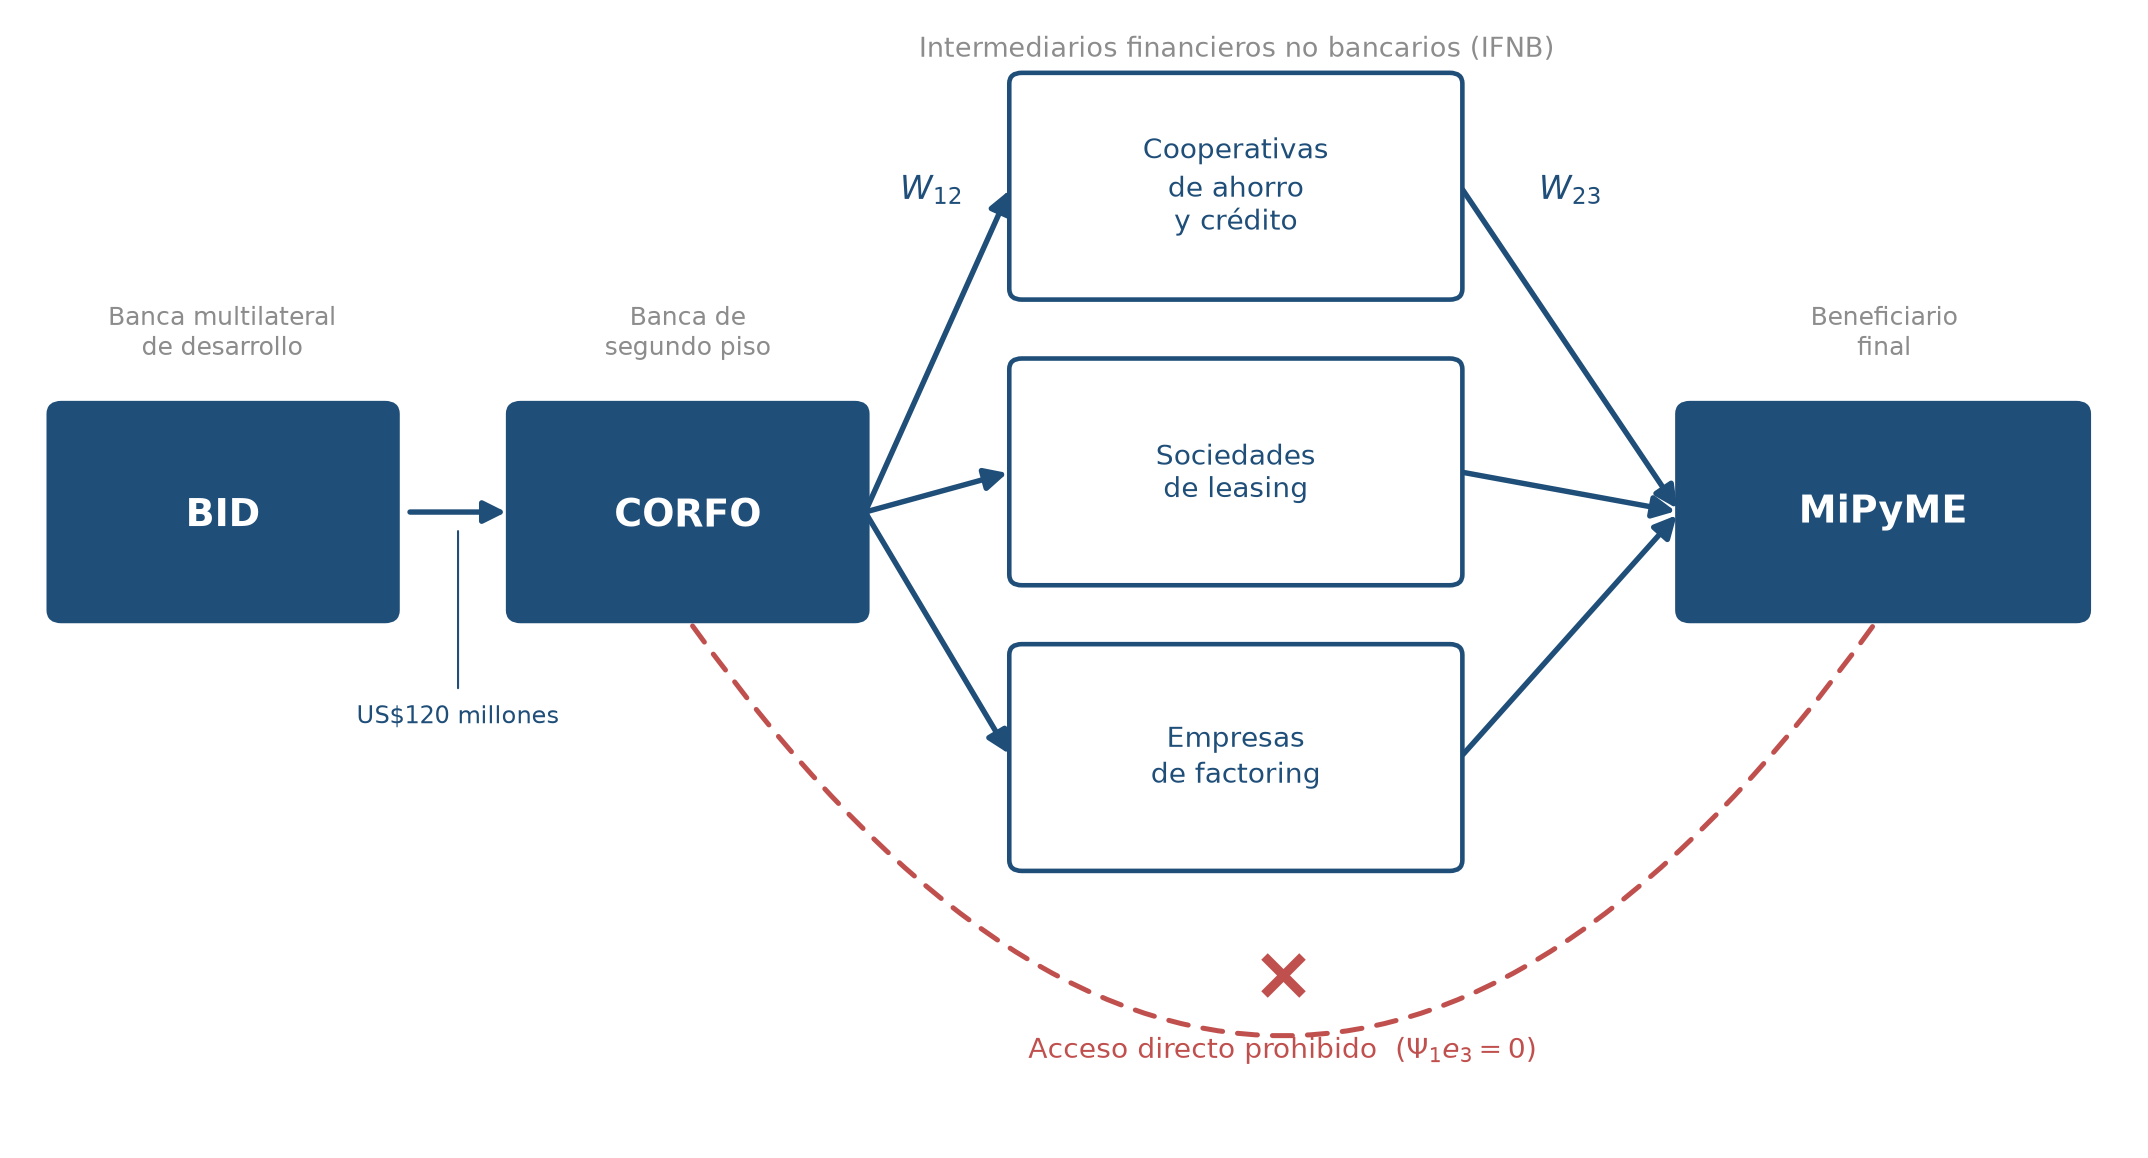
\includegraphics[width=\textwidth]{fig_cadena_corfo.png}
\caption[Cadena institucional del programa Crédito Corfo Mipyme]{Cadena institucional del programa Crédito Corfo Mipyme. El BID aporta el fondeo a CORFO, que actúa como banca de segundo piso y gira recursos ($W_{12}$) hacia tres tipos de intermediario financiero no bancario, los que a su vez colocan crédito ($W_{23}$) en las empresas beneficiarias. El acceso directo de la MiPyME a los recursos de CORFO está prohibido por el diseño del programa, lo que en el modelo se codifica como $\Psi_1 e_3 = 0$. El BID no se modela como agente de la red porque no contrata con los agentes aguas abajo.}
\label{fig:cadena}
\end{figure}

\subsection{Definición de MiPyME y tramos de tamaño}
\label{c3:mipyme}

La sigla MiPyME agrupa a las micro, pequeñas y medianas empresas. En Chile esa clasificación la fija el artículo 2 de la Ley N.º 20.416, conocida como Estatuto Pyme, que segmenta a las empresas según sus ingresos anuales por ventas, servicios y otras actividades del giro en el último año calendario, descontados el IVA y los impuestos específicos, y los expresa en unidades de fomento (UF) \cite{ley_20416_2010}. Bajo ese criterio una empresa es MiPyME cuando sus ventas anuales no superan las 100.000 UF.

La ELE-7, de la que proviene el supuesto de tasa de mercado de la Sección~\ref{c3:tasa-mercado}, emplea una clasificación de cinco tramos que subdivide a la pequeña empresa en dos \cite{ele7_metodologia_2024}. La Tabla~\ref{tab:tramos-tamano} reúne ambas clasificaciones y permite leer los tramos que emplea la Tabla~\ref{tab:ele7-tasas}.

\begin{table}[htbp]
\centering
\caption[Tramos de tamaño de empresa según ventas anuales]{Tramos de tamaño de empresa según ventas anuales en UF, con la correspondencia entre los cinco tramos de la ELE-7 y las categorías del Estatuto Pyme.}
\label{tab:tramos-tamano}
\small
\begin{tabular}{lll}
\hline
Tramo ELE-7 & Ventas anuales (UF) & Categoría de la Ley N.º 20.416 \\
\hline
Micro      & Hasta 2.400                      & Microempresa \\
Pequeña 1  & Más de 2.400 y hasta 5.000       & Pequeña empresa \\
Pequeña 2  & Más de 5.000 y hasta 25.000      & Pequeña empresa \\
Mediana    & Más de 25.000 y hasta 100.000    & Mediana empresa \\
Grande     & Más de 100.000                   & Gran empresa \\
\hline
\end{tabular}
\end{table}

\subsection{Estructura de las dos redes}
\label{c3:estructura}

El caso se modela como un sistema de cuatro agentes distribuidos en dos redes, siguiendo la extensión dual de \citeA{venegas_dual_network_2024} presentada en la Sección~\ref{c24}. La Figura~\ref{fig:redes} resume esta estructura.

\begin{itemize}
    \item Red Tradicional (T). CORFO (1) $\to$ Intermediario/IFNB (2) $\to$ MiPyME (3), con la arista CORFO--MiPyME prohibida, lo que se codifica como $\Psi_1 e_3 = 0$. Corresponde al canal del programa Crédito Corfo Mipyme.
    \item Red Alternativa (A). Banco tradicional (4) $\to$ MiPyME (3), un único par sin restricciones de acceso, que representa la obtención de crédito comercial en el sistema bancario de mercado, fuera del programa.
\end{itemize}

La elección de esta partición responde a dos criterios. Primero, la red Tradicional reproduce la restricción regulatoria que motiva el modelo dual, ya que el acceso al financiamiento subsidiado está mediado obligatoriamente por un intermediario autorizado. Segundo, la MiPyME resulta ser el único agente presente en ambas redes, mientras que CORFO y el IFNB participan solo en T y el banco tradicional solo en A. En consecuencia, la MiPyME es el único agente cuyo portafolio debe repartirse entre canales mediante la partición dual de la Ecuación~\eqref{eq:particion}, y por lo tanto el único que requiere resolver el sistema acoplado.

Junto a esa partición, el Capítulo~\ref{c4} examina una rama contrafactual que corresponde declarar aquí, puesto que es una construcción metodológica y no una descripción del programa. Dicha rama conserva solo tres agentes, a saber CORFO, el intermediario y la MiPyME, de modo que prescinde del banco de mercado. En ella la arista entre CORFO y la MiPyME sigue prohibida en la red Tradicional, mientras que la red Alternativa la habilita, de manera que CORFO puede prestar de forma directa. Su propósito es medir cuánto bienestar deja sobre la mesa el mandato de segundo piso, y por lo tanto no representa ninguna configuración observable del programa. Las cifras que entrega se reportan en la Sección~\ref{c4:prediccion-contrafactual}.

\begin{figure}[htbp]
\centering
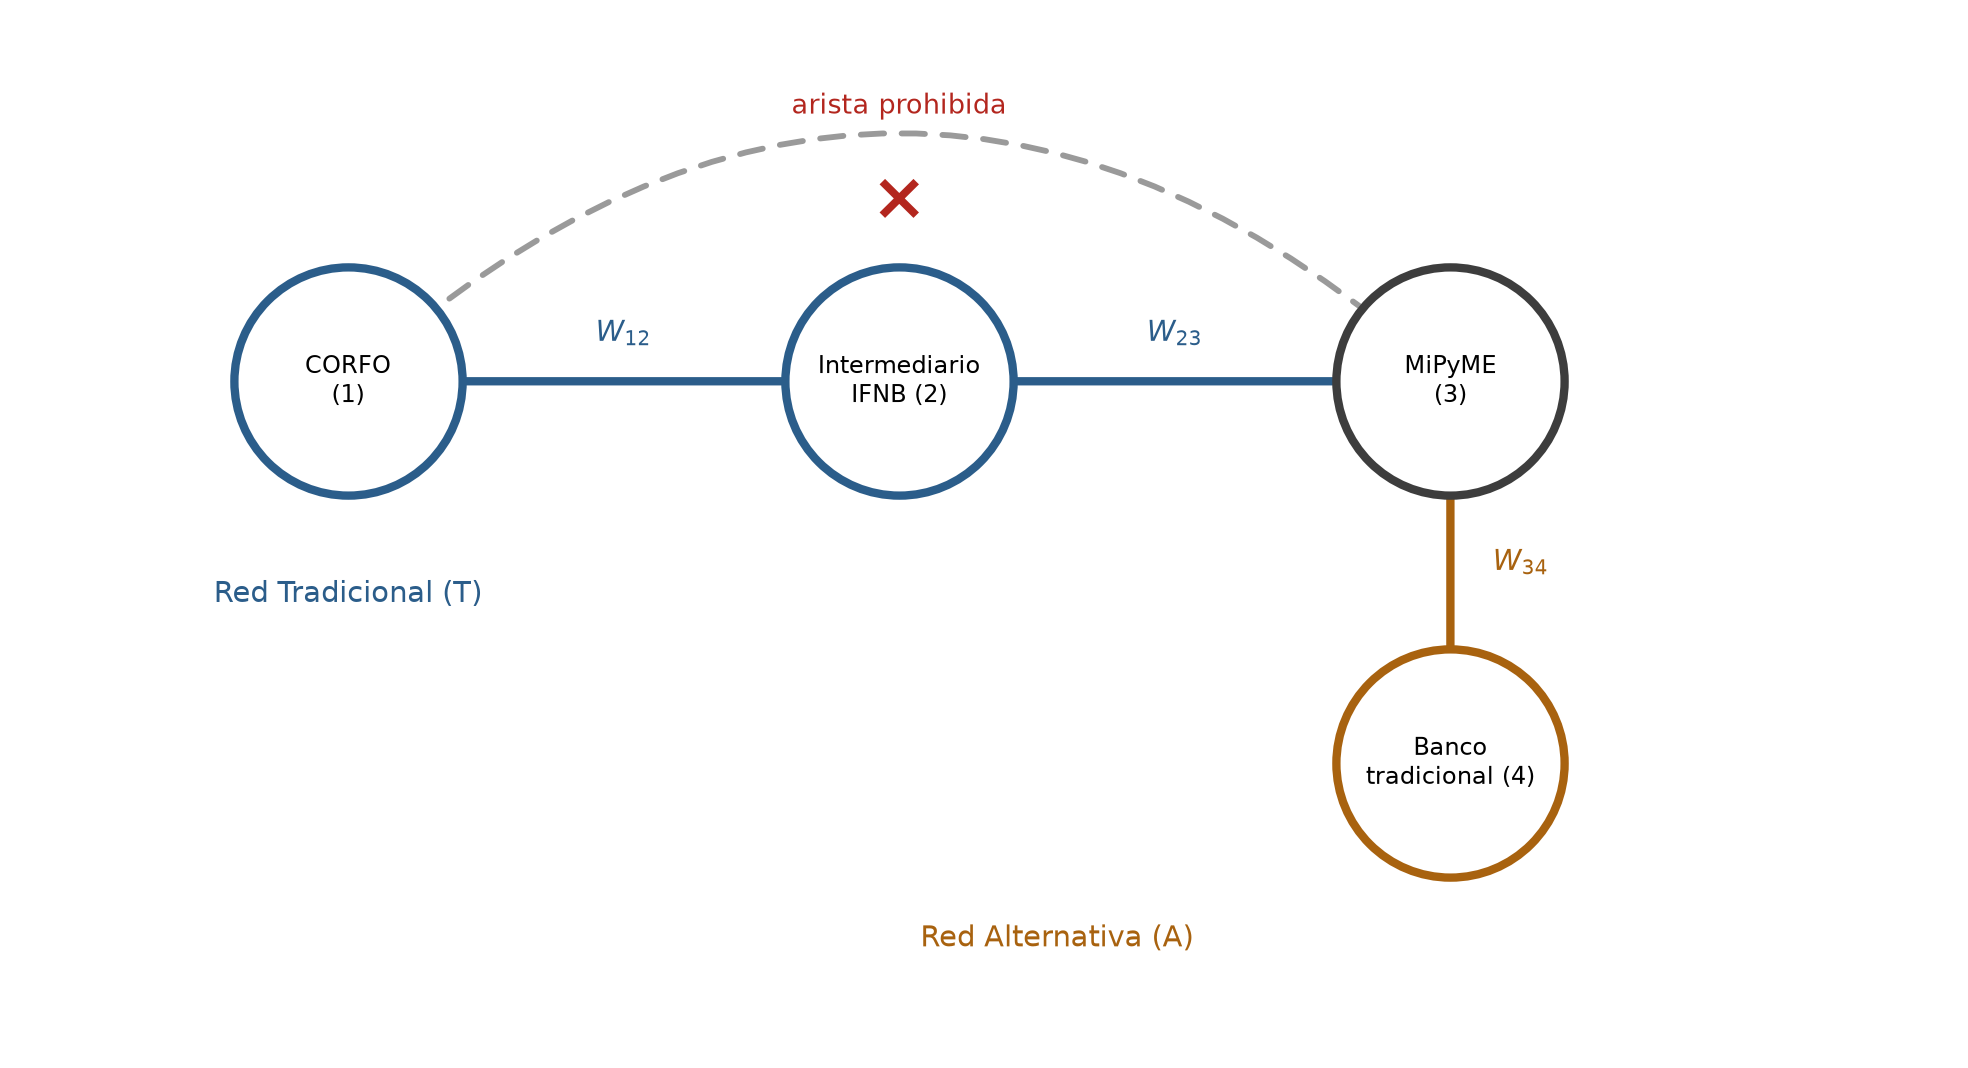
\includegraphics[width=0.85\textwidth]{diagrama_redes.png}
\caption[Estructura de las dos redes del caso de aplicación]{Estructura de las dos redes del caso de aplicación. La red Tradicional (azul) canaliza financiamiento de CORFO hacia la MiPyME a través de un intermediario financiero no bancario, con la arista directa CORFO--MiPyME prohibida. La red Alternativa (naranja) representa el acceso a crédito bancario de mercado. La MiPyME es el único agente presente en ambas redes.}
\label{fig:redes}
\end{figure}

\section{Datos disponibles y método de obtención}
\label{c3:datos}

\subsection[Panel W12 (CORFO a Intermediario/IFNB)]{Panel $W_{12}$ (CORFO $\to$ Intermediario/IFNB)}
\label{c3:panel-w12}

Esta serie se extrajo de las ``Cuentas Públicas Participativas'' anuales de CORFO, disponibles en el repositorio institucional \texttt{repositoriodigital.corfo.cl}, cuya colección 2014--2024 permitió listar y descargar los PDF de cada gestión anual. De los 11 documentos descargados se obtuvo el monto de préstamos otorgados por CORFO a intermediarios financieros no bancarios (IFNB) para los años 2019, 2020 y 2024 \cite{corfo_cuenta_publica_2019,corfo_cuenta_publica_2020,corfo_cuenta_publica_2024} (en 2016 solo se dispone de la cifra de colocaciones a MiPyMEs bajo el programa antecesor Microcrédito, sin el monto mayorista CORFO-IFNB desagregado). En cambio, para el resto de los años esta cifra desagregada no está publicada, y solo se dispone en algunos casos de la cifra agregada de ``colocaciones'' a MiPyMEs, que mezcla flujo nuevo con cartera rotativa (véase la Sección~\ref{c3:limitaciones}).

\subsection[Ausencia de datos para W23 (Intermediario a MiPyME)]{Ausencia de datos para $W_{23}$ (Intermediario $\to$ MiPyME)}
\label{c3:ausencia-w23}

No existe, hasta donde se ha buscado, una fuente pública que reporte esta arista de forma desagregada y comparable entre años. No obstante, el reglamento operativo del programa Crédito Corfo Mipyme (Texto Refundido, punto 19, ``Justificación de la utilización de los préstamos otorgados a los IFNB'') \cite{corfo_reglamento_credito_mipyme} revela que CORFO sí recibe internamente, mes a mes y por operación individual, tanto la tasa de interés como el saldo de capital vigente de cada crédito. Dicha información resolvería directamente este vacío, aunque no es pública y solo sería accesible a través de un contacto institucional. Actualmente se encuentran en curso conversaciones con dicho contacto para evaluar su disponibilidad.

\subsection{Datos para la red Alternativa}
\label{c3:datos-alternativa}

Se utilizan dos fuentes públicas. La primera es la Dirección de Presupuestos (DIPRES), organismo dependiente del Ministerio de Hacienda que elabora el presupuesto del sector público y realiza el monitoreo y seguimiento de los programas públicos, entre ellos el programa Crédito Corfo Mipyme. Su Informe de Detalle de Programas Sociales con cierre a diciembre de 2021 \cite{dipres_detalle_2021} reporta la tasa de interés mayorista CORFO$\to$IFNB (4,23\%--4,73\% anual) y cuyo Informe de Monitoreo 2021 \cite{dipres_monitoreo_2021} reporta el spread de la tasa a cliente final IFNB respecto al benchmark de mercado ACHEF/EFA ($-7$ a $-10$ puntos porcentuales). La segunda es la ELE-7 (Séptima Encuesta Longitudinal de Empresas), cuyos microdatos completos \cite{ele7_microdatos_2024} (\texttt{ele7-full.csv}, 6.592 empresas) permiten obtener la tasa de interés del crédito de mayor monto aprobado en 2022 (variable \texttt{B066}), segmentada por tamaño de empresa (variable \texttt{TAMANO}) y anualizada según periodicidad reportada (variables \texttt{B067}/\texttt{B068}). Complementariamente, el informe oficial de resultados de la misma encuesta \cite{ele7_informe_2024} reporta la tasa de rechazo condicional a la solicitud de crédito por tamaño de empresa.


Ninguna de estas dos fuentes se distribuye junto con el código que acompaña a este trabajo, tanto por su tamaño como por sus condiciones de uso, de modo que conviene dejar indicada la vía de obtención de cada una. Los microdatos de la ELE-7 se descargan como archivo único desde el sitio del Ministerio de Economía, Fomento y Turismo, mientras que el Informe de Monitoreo y el Informe de Detalle de Programas Sociales se obtienen desde la biblioteca digital de DIPRES. La dirección exacta de cada documento queda registrada en su entrada de la bibliografía.

El Anexo~\ref{anexo:fuentes} resume las fuentes consultadas y el insumo que aporta cada una.

\section{Supuestos del modelo para las variables no observadas}
\label{c3:supuestos}

\subsection[Supuesto para W23. Tasa subsidiada del canal Tradicional]{Supuesto para $W_{23}$. Tasa subsidiada del canal Tradicional}
\label{c3:supuesto-w23}

Se asume que la tasa de interés que los IFNB cobran a la MiPyME bajo el programa Crédito Corfo Mipyme se ubica entre 7 y 10 puntos porcentuales por debajo del benchmark de mercado (ACHEF/EFA), según reporta DIPRES en su Informe de Monitoreo 2021 del programa \cite{dipres_monitoreo_2021}. Tomando como benchmark de mercado la tasa mediana observada para empresas de menor tamaño, que va de 14\% a 15,4\% anual (Sección~\ref{c3:tasa-mercado}), ese descuento sitúa la tasa subsidiada entre 4\% y 8,4\% anual. Una segunda referencia, independiente de la anterior, es la tasa mayorista CORFO$\to$IFNB, que \citeA{dipres_detalle_2021} reporta entre 4,23\% y 4,73\% anual y que opera como piso, ya que el IFNB traspasa el subsidio casi íntegro a la MiPyME y agrega solo un margen operativo menor, en línea con el rol de ``banca de segundo piso'' que describe CORFO para este programa.

Sobre esas dos referencias se adopta como supuesto de trabajo el rango de 3\% a 6\% anual, que es el que emplea la corrida de la Sección~\ref{c4:prediccion}. Corresponde declarar con precisión su estatus, dado que no se deduce de ninguna de las dos referencias sino que las resume de forma deliberadamente amplia, de modo que su extremo inferior queda por debajo de la tasa mayorista y su extremo superior por debajo del máximo que admite el descuento declarado.

De esa amplitud se sigue una consecuencia que el supuesto debe hacer explícita. El margen del intermediario es la diferencia entre la tasa subsidiada y la mayorista, de manera que con los intervalos anteriores recorre desde $-1{,}73$ hasta $+1{,}77$ puntos porcentuales, y solo el 50,7\% del área del rectángulo que forman ambos intervalos deja un margen positivo, proporción que sobre la rejilla del barrido corresponde a 384 de las 768 combinaciones. En la mitad restante el modelo predice que el intermediario no coloca y que el programa no opera, situación que no describe al programa aquí representado. Por esa razón la corrida de la Sección~\ref{c4:prediccion-reparto} descarta de forma explícita las combinaciones de margen negativo, descarte que forma parte del supuesto mientras no exista una fuente que reporte directamente la tasa cobrada a la MiPyME.

\subsection[Supuesto para la red Alternativa. Tasa de mercado M34]{Supuesto para la red Alternativa. Tasa de mercado $M_{34}$}
\label{c3:tasa-mercado}

$M_{34}$ representa, en la notación del modelo, la creencia de retorno esperado entre la MiPyME y un banco tradicional si negociaran un contrato de crédito en la red Alternativa. No se dispone de una fuente que mida directamente esta creencia bilateral, por lo que se la aproxima mediante la tasa de interés de mercado efectivamente pagada por empresas de tamaño comparable, bajo el supuesto de que dicha tasa refleja razonablemente el costo/retorno que ambas partes anticiparían en una negociación real. Para la tasa de mercado que enfrentaría la MiPyME en el canal bancario tradicional (sin fondeo CORFO), se utiliza la tasa de interés anualizada del crédito de mayor monto aprobado en 2022, calculada directamente de los microdatos de la ELE-7 \cite{ele7_microdatos_2024} (variable B066 segmentada por TAMANO, con anualización explícita de los casos reportados en base mensual). Se reporta la mediana en preferencia a la media, dado que esta última se ve distorsionada por un pequeño número de casos atípicos en el segmento de empresas grandes. La Figura~\ref{fig:ele7-distribucion} documenta esa elección a partir de la distribución completa de las tasas y no solo de sus resúmenes.

\begin{figure}[htbp]
\centering
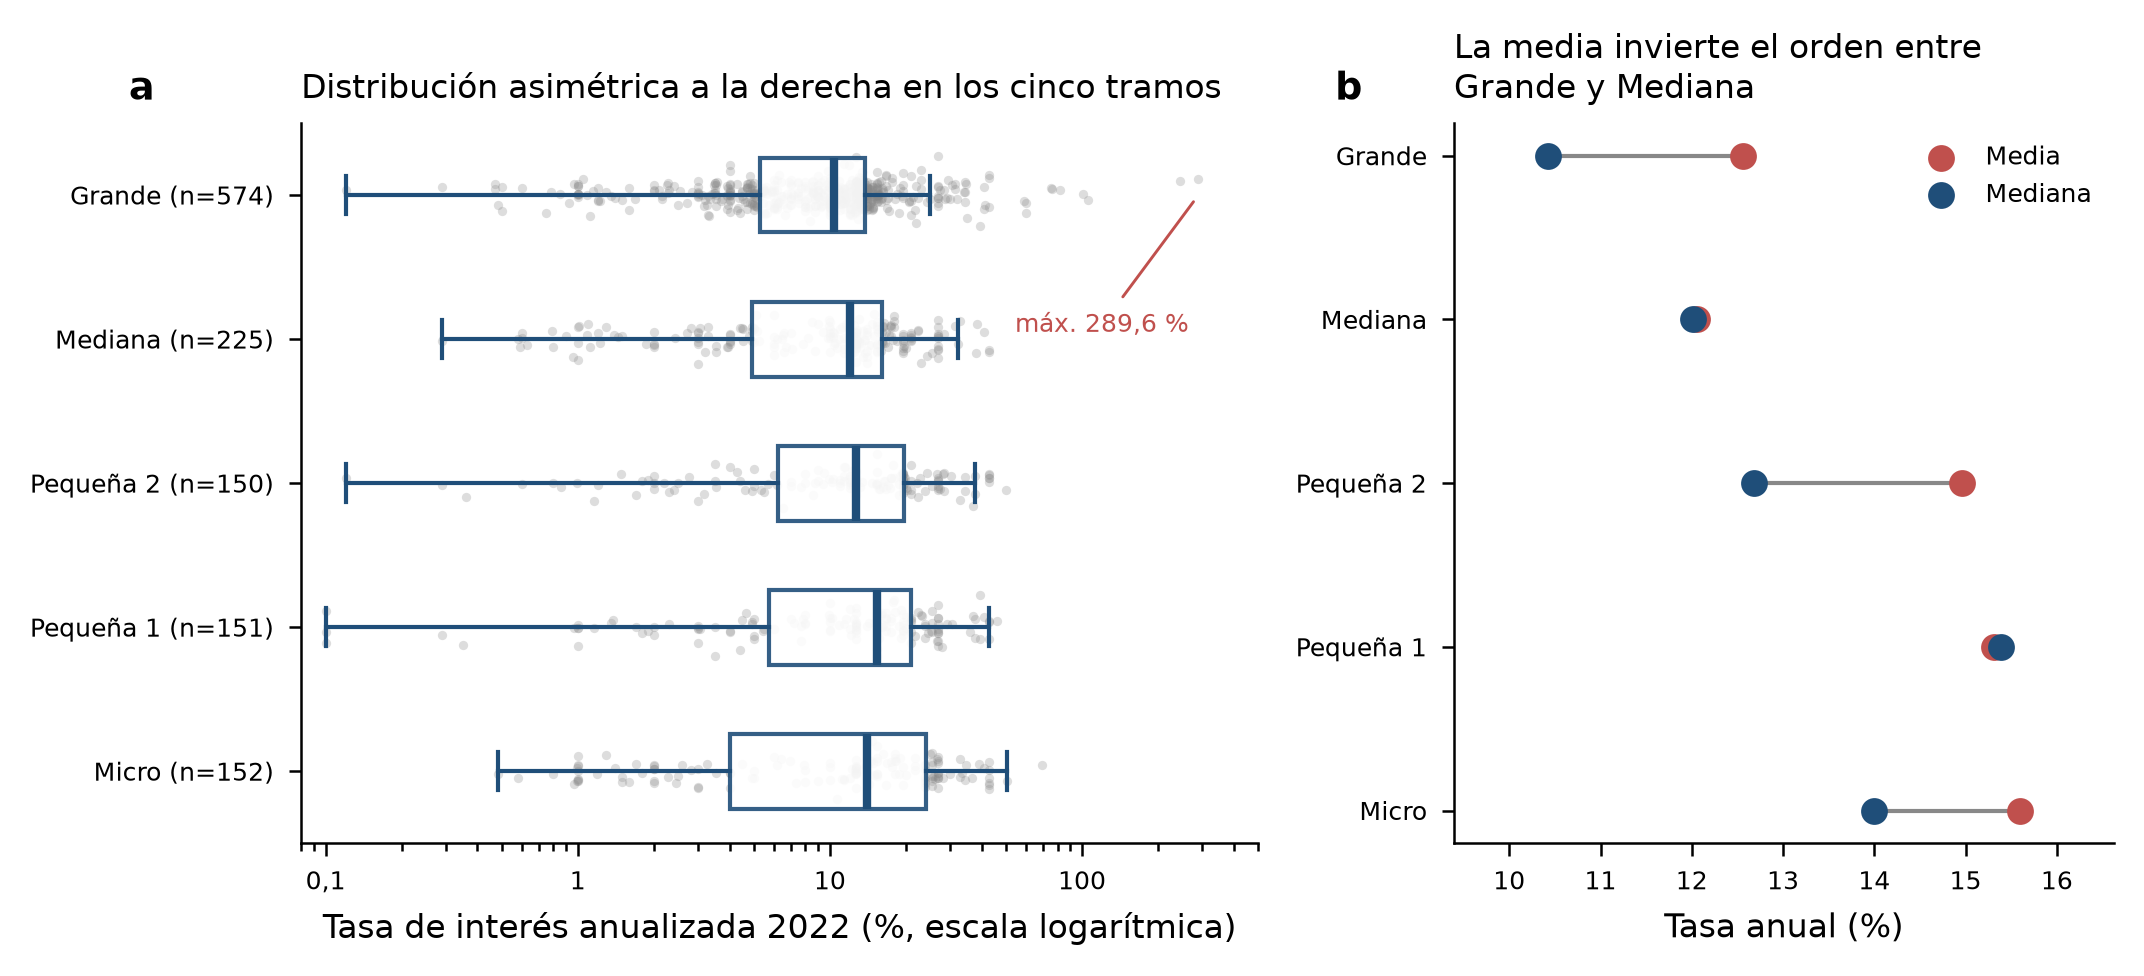
\includegraphics[width=\textwidth]{fig_ele7_distribucion_tasas.png}
\caption[Distribución de la tasa de interés anualizada 2022 por tamaño de empresa]{Distribución de la tasa de interés anualizada del crédito de mayor monto aprobado en 2022, por tramo de tamaño de empresa. Elaboración propia a partir de los microdatos de la ELE-7 \cite{ele7_microdatos_2024} (variable \texttt{B066} segmentada por \texttt{TAMANO}), sobre las $1.252$ empresas que reportan tasa. El panel (a) usa escala logarítmica para hacer visible el rango completo de los datos, con cada punto gris una empresa y la caja los cuartiles. El panel (b) contrasta mediana y media por tramo.}
\label{fig:ele7-distribucion}
\end{figure}

El panel (a) de la Figura~\ref{fig:ele7-distribucion} muestra que la distribución es asimétrica a la derecha en los cinco tramos, con coeficientes de asimetría que van de $0{,}67$ en Pequeña~1 a $9{,}92$ en Grande. En una distribución con esta forma la media deja de representar al caso típico, porque las observaciones de la cola larga la desplazan hacia arriba sin que exista una cola equivalente que compense hacia abajo. El tramo Grande concentra el problema, ya que registra $41$ observaciones atípicas superiores según el criterio de rango intercuartílico y una tasa máxima de $289{,}6\%$ anual.

El panel (b) hace explícita la consecuencia para el supuesto que aquí interesa. Medida por la mediana, la tasa del tramo Grande ($10{,}43\%$) es menor que la del tramo Mediana ($12{,}01\%$), lo que concuerda con la relación esperada entre tamaño de empresa y costo del crédito. Medida por la media, en cambio, el tramo Grande ($12{,}56\%$) aparece por sobre el tramo Mediana ($12{,}06\%$), es decir, el orden se invierte. Esa inversión no refleja un fenómeno económico sino la influencia de unas pocas observaciones extremas, ya que basta con excluir la observación máxima de las $574$ del tramo Grande para que su media caiga de $12{,}56\%$ a $12{,}07\%$ y la inversión prácticamente desaparezca. La media recortada al $10\%$ confirma el diagnóstico, puesto que restituye el orden esperado con $10{,}01\%$ en Grande frente a $11{,}19\%$ en Mediana.

Por lo tanto, la mediana es el estimador adecuado en este caso. Es insensible a las observaciones extremas que distorsionan la media, preserva el ordenamiento económico entre tramos y no depende de una decisión arbitraria sobre qué observaciones recortar.

\begin{table}[htbp]
\centering
\caption[Tasa de interés mediana anual 2022 por tamaño de empresa (ELE-7)]{Tasa de interés anualizada mediana del crédito de mayor monto aprobado en 2022, por tamaño de empresa. Elaboración propia a partir de los microdatos de la ELE-7 \cite{ele7_microdatos_2024} (variable \texttt{B066} segmentada por \texttt{TAMANO}).}
\label{tab:ele7-tasas}
\begin{tabular}{lcc}
\hline
Tramo ELE-7 & Tasa mediana anual 2022 & $n$ \\
\hline
Grande      & 10,43\% & 574 \\
Mediana     & 12,01\% & 225 \\
Pequeña 2   & 12,68\% & 150 \\
Pequeña 1   & 15,39\% & 151 \\
Micro       & 14,00\% & 152 \\
\hline
\end{tabular}
\end{table}

Se adopta, por lo tanto, el rango 14\%--15,4\% (segmentos Pequeña~1 y Micro) como supuesto de $M_{34}$ para la MiPyME en la red Alternativa. La Tabla~\ref{tab:ele7-tasas} muestra una tendencia general de mayor tasa a menor tamaño (Grande 10,43\% frente a Pequeña~1 15,39\%); sin embargo, esta relación no es estrictamente monotónica, ya que Micro (14,00\%) queda levemente por debajo de Pequeña~1 (15,39\%). Dicha diferencia puede reflejar más bien el tamaño de muestra reducido ($n=151$ y $n=152$ respectivamente) que un efecto económico real, por lo que debe reportarse sin forzar una lectura estrictamente monotónica.

\subsection[Supuesto para la fricción de acceso lambda A]{Supuesto para la fricción de acceso $\lambda_A$}
\label{c3:supuesto-lambda}

$\lambda_A$ es, en el modelo dual de la Ecuación~\eqref{eq:utilidad-dual}, el parámetro que determina cuán costoso o restringido resulta para la MiPyME acceder a la red Alternativa en comparación con la red Tradicional, y por lo tanto gobierna cómo la MiPyME reparte su portafolio entre ambos canales. Un $\lambda_A$ alto implica que, aun si el modelo predijera una tasa competitiva en la red Alternativa, la MiPyME en la práctica no podría aprovecharla con facilidad. Como segunda ancla, independiente de la anterior, se utiliza la tasa de rechazo condicional a la solicitud de crédito reportada en el informe oficial de resultados de la ELE-7 \cite{ele7_informe_2024}, que llega a 15\% para MiPyMEs frente a 3\% para empresas grandes (cinco veces mayor). Adicionalmente, 111 de las 1.018 empresas que necesitaban crédito pero nunca lo solicitaron declaran autocensura, una población disjunta de las 819 empresas que sí solicitaron crédito. Esta brecha de acceso, combinada con la brecha de tasa anterior, sustenta por lo tanto el supuesto de que $\lambda_A$ es sustancialmente mayor que la fricción de acceso a la red Tradicional para el agente MiPyME.

\section{Diagnóstico de factibilidad empírica}
\label{c3:diagnostico}

\subsection{Aplicación del Teorema 5 al caso de estudio}
\label{c3:teorema5-aplicado}

Con $n=4$ agentes (CORFO, Intermediario, MiPyME y Banco tradicional), la cota del Teorema 5 recogida en la Ecuación~\eqref{eq:teorema5} exige un mínimo de $m \geq \lceil 4\ln 4\rceil = 6$ observaciones independientes para que la estimación de $\Sigma$ no degrade sustancialmente la convergencia del algoritmo de negociación bilateral. Sin embargo, según el levantamiento de la Sección~\ref{c3:panel-w12}, los años en que se dispone simultáneamente de $W_{12}$ y $W_{23}$ son 2019, 2020 y 2024, a los que se agrega 2016 únicamente con la cifra de colocaciones del programa antecesor. Esas tres observaciones quedan por debajo del mínimo de seis que exige la Ecuación~\eqref{eq:teorema5}. La restricción es aún más severa por la vía de la Proposición~1, que opera sobre las diferencias $\Delta W(t) = W(t+1)-W(t)$, ya que de esos tres años solo el par 2019--2020 es consecutivo y aporta, por lo tanto, una única diferencia utilizable frente a los seis parámetros libres de $\Sigma$ en la red Tradicional. Tomando las dos redes en conjunto, que es el sistema de cuatro agentes sobre el que está definida $\Sigma$, no hay ninguna diferencia utilizable, puesto que ningún año dispone de todas sus aristas.

\subsection[Identificabilidad de Sigma en la red del programa]{Identificabilidad de $\Sigma$ en la red del programa}
\label{c3:identificabilidad}

La cota del Teorema 5 responde cuántos periodos se necesitan, pero presupone que $\Sigma$ puede recuperarse en principio. Esa condición se evaluó de forma independiente para la red del programa, mediante el rango de la información del estimador de la Proposición~1 de \citeA{jalan_incentive-aware_2024}. El estimador de la Ecuación~\eqref{eq:prop1} actúa sobre el residuo $\Sigma\,\Delta W + \Delta W\,\Sigma$ evaluado en las aristas permitidas, de modo que el rango del mapa lineal que lleva $\Sigma$ a ese residuo indica cuántas de sus $n(n+1)/2$ entradas libres quedan determinadas. La matriz $\Sigma$ es identificable cuando el rango iguala ese número, o cuando falta una sola dirección y su traza no es nula, ya que la normalización $\operatorname{tr}(\Sigma)=1$ solo puede fijar una.

\paragraph{Caso de tres agentes.}
Sea la cadena CORFO (1), Intermediario (2) y MiPyME (3), con la arista 1--3 prohibida. Si $a=\Delta W_{12}$ y $b=\Delta W_{23}$ denotan los cambios de los dos contratos entre un periodo y el siguiente, el residuo en las dos aristas permitidas es
\begin{equation}
\label{eq:residuo-cadena}
\begin{aligned}
R_{12} &= a\,(\Sigma_{11}+\Sigma_{22}) + b\,\Sigma_{13},\\
R_{23} &= b\,(\Sigma_{22}+\Sigma_{33}) + a\,\Sigma_{13}.
\end{aligned}
\end{equation}
Solo intervienen cuatro de las seis entradas de $\Sigma$. Las covarianzas $\Sigma_{12}$ y $\Sigma_{23}$ no figuran en ninguna ecuación y las varianzas aparecen únicamente a través de sumas. En cambio, $\Sigma_{13}$ aparece de forma aislada, por lo que queda determinada aunque el contrato directo 1--3 esté prohibido. En consecuencia, el rango es 3 de 6 grados de libertad. La normalización de la traza no basta para cerrar la brecha, porque faltan tres direcciones y no una.

\paragraph{Estructura bipartita de la red de registros de CORFO.}
La red que entregan los registros de CORFO, formada por CORFO, los $k$ intermediarios y la MiPyME, es bipartita. Un lado lo integran CORFO y la MiPyME, y el otro lado los intermediarios, de modo que toda arista une agentes de lados distintos y ninguna une agentes del mismo lado. Como consecuencia, el residuo de cada arista involucra solo covarianzas entre agentes del mismo lado, y las covarianzas entre lados, que son las de las propias aristas, no intervienen en ninguna ecuación. Este resultado se limita a esa red y no al sistema completo de las dos redes, donde el Banco participa solo en la red Alternativa.

La Tabla~\ref{tab:rango-bipartita} muestra que el déficit de rango crece como $2k+1$ con el número de intermediarios. En consecuencia, agregar intermediarios no repara la identificación. Tampoco lo hace aumentar el número de periodos, ya que cada periodo adicional aporta ecuaciones de la misma forma que la Ecuación~\eqref{eq:residuo-cadena}. La limitación es, por lo tanto, estructural y no muestral.

\begin{table}[htbp]
\centering
\caption[Rango de identificación en la red bipartita de CORFO]{Rango de la información del estimador de la Proposición~1 en la red CORFO, $k$ intermediarios y MiPyME, con la arista CORFO--MiPyME prohibida. Elaboración propia.}
\label{tab:rango-bipartita}
\small
\begin{tabular}{cccccc}
\hline
$k$ & Agentes $n$ & Grados de libertad & Rango & Déficit & Identificable \\
\hline
1 & 3 & 6  & 3  & 3  & No \\
2 & 4 & 10 & 5  & 5  & No \\
3 & 5 & 15 & 8  & 7  & No \\
4 & 6 & 21 & 12 & 9  & No \\
5 & 7 & 28 & 17 & 11 & No \\
6 & 8 & 36 & 23 & 13 & No \\
\hline
\end{tabular}
\end{table}

\paragraph{Entradas recuperables.}
En las topologías con uno y con tres intermediarios, las únicas entradas determinadas son las covarianzas entre agentes que no contratan entre sí, esto es, $\Sigma_{13}$ entre CORFO y la MiPyME y las covarianzas entre pares de intermediarios. No quedan determinadas, de manera individual, las varianzas propias ni las covarianzas a lo largo de las aristas observadas. El detalle por tipo de entrada se presenta en la Sección~\ref{anexo:entradas} del Anexo.

\paragraph{Extensión de diseño que completa la identificación.}
El modelo dual tiene tres aristas estructurales, CORFO--Intermediario e Intermediario--MiPyME en la red Tradicional y Banco--MiPyME en la red Alternativa. Las aristas Intermediario--Banco y CORFO--Banco no pertenecen al modelo vigente y se evaluaron como una extensión de diseño. La Tabla~\ref{tab:rango-extension} resume el resultado con tres intermediarios. Solo la arista Intermediario--Banco rompe la bipartición, puesto que une dos agentes que quedan del mismo lado. La arista CORFO--Banco cruza de lado y no la rompe, pero el rango completo se alcanza únicamente cuando ambas están presentes.

\begin{table}[htbp]
\centering
\caption[Rango de identificación con aristas bancarias adicionales]{Rango de la información del estimador de la Proposición~1 con tres intermediarios al incorporar el Banco y las aristas Intermediario--Banco y CORFO--Banco. Elaboración propia.}
\label{tab:rango-extension}
\small
\begin{tabular}{lcccc}
\hline
Red evaluada & Grados de libertad & Rango & Déficit & Identificable \\
\hline
Registros de CORFO (sin Banco)             & 15 & 8  & 7 & No \\
Con Banco--MiPyME                          & 21 & 12 & 9 & No \\
Con Banco--MiPyME y CORFO--Banco           & 21 & 12 & 9 & No \\
Con Banco--MiPyME e Intermediario--Banco  & 21 & 18 & 3 & No \\
Con ambas aristas bancarias                & 21 & 21 & 0 & Sí \\
\hline
\end{tabular}
\end{table}

En términos prácticos, las aristas Intermediario--Banco y CORFO--Banco corresponden al fondeo bancario de los propios intermediarios y a las líneas que CORFO coloca a través de bancos comerciales, respectivamente. Incorporarlas supone una decisión de diseño sobre el modelo y requiere series que hoy no están disponibles, por lo que se reportan aquí como condición de identificación y no como dato faltante del modelo vigente.

\subsection{Relación con el algoritmo de negociaciones y el Teorema 4}
\label{c3:algoritmo1-aplicado}

El Teorema 1, recogido en la Ecuación~\eqref{eq:teorema1}, resuelve el punto estable de forma exacta mediante un sistema lineal, y para el caso de estudio con las restricciones estructurales ya conocidas ese sistema $Z_F$ es de baja dimensión, por lo que se resolvería exactamente y sin necesidad de iterar. En consecuencia, el mecanismo directo para calcular el $W_{23}$ predicho a partir de los supuestos de la Sección~\ref{c3:supuestos}, tarea que corresponde al procedimiento de la Sección~\ref{c3:calibracion}, es el Teorema 1 y no el Algoritmo~\ref{alg:negociaciones}.

El Algoritmo~\ref{alg:negociaciones}, en cambio, cobra relevancia práctica en un problema distinto y de mayor escala, que es la implementación completa del modelo dual mediante la capa de acoplamiento T/A. Ahí, el sistema conjunto que resuelve la partición de la Ecuación~\eqref{eq:particion} para la MiPyME se beneficia de un mecanismo descentralizado, en el que cada par de agentes negocia usando solo su propio precio vigente y sin necesidad de conocer de antemano toda la red, tal como lo haría un agente real. Es en ese contexto, y no en el cálculo puntual de este caso, donde el factor de amortiguación $\eta$ y su cota de convergencia, dada por la Ecuación~\eqref{eq:eta}, pasan a ser relevantes en la práctica.

\section{Procedimiento de calibración}
\label{c3:calibracion}

Establecida la factibilidad, la calibración y la aplicación del modelo sobre el
caso seleccionado comprenden las tareas siguientes.

\begin{enumerate}
    \item Construcción de los primitivos $(M,\Gamma,\Sigma)$ a partir de las
    series levantadas y de los supuestos declarados en la
    Sección~\ref{c3:supuestos}, respetando las restricciones de acceso
    $\Psi_i$ que impone la estructura del caso.
    \item Cálculo del punto estable mediante el sistema lineal de la
    Ecuación~\eqref{eq:teorema1}, del que se obtiene el tamaño de contrato
    predicho para cada par de agentes, en particular $W_{23}$, y el vector de
    precios asociado.
    \item Contraste de las predicciones del modelo calibrado, tanto de
    recuperación de bienestar como de reparto de actividad entre la red
    Tradicional y la red Alternativa, con la evidencia observada en el caso
    real, lo que responde las preguntas de investigación formuladas en la
    Sección~\ref{c1:preguntas}.
    \item Análisis de sensibilidad de los resultados ante variaciones en los
    parámetros del modelo dual, en particular el beneficio de transparencia
    $\tau$ y la fricción de acceso $\lambda_A$ de la
    Ecuación~\eqref{eq:utilidad-dual}, dado que ninguno de los dos se observa
    directamente en los datos.
\end{enumerate}

Por el resultado de identificabilidad discutido en la
Sección~\ref{c24:identificacion}, la calibración reporta como no
identificadas las varianzas propias y las covarianzas a lo largo de las aristas
observadas, en lugar de estimarlas, ya que la estructura bipartita de la red del
programa no permite recuperarlas aunque aumente el volumen de datos. En cambio,
la covarianza $\Sigma_{13}$ entre CORFO y la MiPyME sí queda determinada.

\section{Limitaciones}
\label{c3:limitaciones}

\begin{enumerate}
    \item Ambigüedad entre flujo y saldo. En varios años, la cifra reportada de ``colocaciones'' a MiPyMEs mezcla desembolso nuevo con cartera rotativa de años anteriores, lo que impide tratarla como $W_{23}(t)$ en el sentido estricto del modelo, es decir, como una fotografía del contrato vigente en un punto estable.
    \item Asimetría de agregación entre redes. $W_{12}$ proviene de un programa e institución identificables, mientras que los supuestos de la red Alternativa provienen de promedios de mercado a nivel nacional (ELE-7), no de una relación bilateral banco--MiPyME específica.
    \item Identificabilidad estructural de $\Sigma$. La red del programa es bipartita, de modo que el programa semidefinido de la Ecuación~\eqref{eq:prop1} no determina las varianzas propias ni las covarianzas a lo largo de las aristas observadas, independientemente del volumen de datos disponible, según se argumenta en la Sección~\ref{c24:identificacion} y se cuantifica en la Sección~\ref{c3:identificabilidad}. Solo las covarianzas entre agentes que no contratan entre sí, como $\Sigma_{13}$, quedan determinadas.
    \item Cobertura incompleta del panel CORFO. Existen años cuyos datos desagregados de este programa no están publicados. Esto significa que los años disponibles no son una muestra representativa del período completo, lo que introduce un sesgo de selección no cuantificado.
\end{enumerate}

% cap4.tex

\chapter{Análisis}
\label{c4}

Este capítulo inicia el análisis empírico del trabajo. Dado que la validación
que se persigue consiste en trasladar a un caso real un método que ya fue
aplicado a datos reales por sus propios autores, el análisis comienza por
reconstruir con precisión ese ejercicio de referencia, que es la aplicación de
\citeA{jalan_incentive-aware_2024} a la red de comercio internacional de la
OCDE. Sobre esa base se documenta después el levantamiento de datos realizado
para el programa Crédito Corfo Mipyme y se contrastan ambos casos, de modo que
la distancia entre uno y otro quede medida y no simplemente afirmada. El
capítulo cierra delimitando qué parte del análisis ya es concluyente con la
información disponible y qué parte queda condicionada a la entrega de datos
solicitada a CORFO.

\section{El ejercicio empírico de referencia. El caso de la OCDE}
\label{c4:ocde}

\subsection{Qué pregunta responde el ejercicio}
\label{c4:ocde-pregunta}

La aplicación empírica del modelo invierte la relación habitual entre datos y
teoría. Los datos no entran para alimentar un modelo que luego produce una red,
sino que la red observada es el dato de entrada y lo que se infiere son las
creencias de riesgo de los agentes, resumidas en la matriz de covarianzas
$\Sigma$. Esa inversión es la razón de ser del ejercicio, ya que $\Sigma$ no es
observable en ninguna fuente, mientras que la red de contratos sí lo es cuando
existe un registro de transacciones bilaterales.

El alcance de lo que puede inferirse está acotado de antemano. Según el
resultado de no identificabilidad recogido en la Sección~\ref{c24:identificacion},
una red $W$ dada no permite separar la terna de creencias $(M,\Gamma,\Sigma)$,
porque para cualquier par admisible de $\Gamma$ y $\Sigma$ existe un $M$ que
reproduce exactamente la misma red, y esa ambigüedad persiste aunque se observen
muchas redes generadas con los mismos $\Sigma$ y $\Gamma$. Por lo tanto el
ejercicio no pretende recuperar las creencias completas, sino únicamente
$\Sigma$ normalizada, bajo los supuestos de homogeneidad que se detallan más
adelante.

Esto explica por qué el conjunto de datos escogido es una red de comercio
internacional y no, por ejemplo, una cartera de créditos. El método exige una
magnitud bilateral que pueda leerse como el tamaño de un contrato entre dos
partes, medida repetidamente en el tiempo sobre el mismo conjunto de agentes y
disponible para prácticamente todos los pares posibles. El comercio bilateral
cumple las tres condiciones de manera natural.

\subsection{Los datos, su origen y su volumen}
\label{c4:ocde-datos}

Los datos provienen de las estadísticas de comercio internacional que publica la
OCDE en su portal estadístico, y cubren el comercio bilateral entre 46 economías
grandes, entre las que se incluyen las quince mayores del mundo por producto
interno bruto. La medición es trimestral y abarca desde el primer trimestre de
2010 hasta el segundo trimestre de 2022, lo que equivale a 50 trimestres.

La construcción del peso de cada arista merece atención porque es una decisión
metodológica y no un detalle de formato. El peso del par $\{i,j\}$ se define como
la suma de los flujos de $i$ hacia $j$ y de $j$ hacia $i$, de modo que la matriz
$W$ resulta simétrica y hay una sola cifra por par, tal como exige el punto
estable del modelo, en el que ambas partes acuerdan la misma cantidad. Dado que
no existe registro de comercio de un país consigo mismo, la red no tiene lazos
propios, y esa ausencia no se trata como dato faltante sino como arista
prohibida, mediante la extensión de la Proposición~1 al caso de aristas
prohibidas.

El volumen resultante se puede precisar. Con 46 agentes hay 1.035 pares
posibles, y con 50 trimestres se obtienen 49 matrices de diferencias
$\Delta W(t)$, de manera que el estimador dispone de 50.715 observaciones de par
por período frente a los 1.081 parámetros libres de $\Sigma$, es decir cerca de
47 ecuaciones por parámetro. La revisión directa del repositorio oficial del
artículo confirma las propiedades estructurales que el modelo supone, ya que las
49 matrices son exactamente simétricas y de diagonal nula, el 98,50~\% de las
entradas fuera de la diagonal es distinto de cero, 959 de los 1.035 pares son no
nulos en los 49 períodos y un solo par permanece en cero durante todo el
horizonte. La red es, en la práctica, completa.

Conviene registrar también cómo se recolectaron esos datos, porque es el punto
en que el caso de referencia y el caso chileno se separan desde el principio. La
recolección consistió en una única descarga desde un repositorio estadístico
internacional que ya publica la información organizada como panel, con
periodicidad uniforme, cobertura homogénea y una sola unidad de medida.

\subsection{El procedimiento aplicado a esos datos}
\label{c4:ocde-procedimiento}

El procedimiento, tal como está implementado en el repositorio oficial, se
compone de cinco pasos encadenados.

\begin{enumerate}
    \item Construcción de la secuencia de redes $W(t)$ y de sus diferencias
    $\Delta W(t)$ entre trimestres consecutivos.
    \item Proyección de cada diferencia con las matrices $\Psi_i$ de la
    topología, operación que anula las entradas correspondientes a aristas
    prohibidas y que en este caso solo afecta a la diagonal.
    \item Resolución del programa semidefinido de la Proposición~1, recogido en
    la Ecuación~\eqref{eq:prop1}, sobre las 49 diferencias, usando el solver SCS
    con cincuenta mil iteraciones, lo que según los propios autores toma del
    orden de treinta minutos.
    \item Regularización de la solución sumando $5\times 10^{-4}$ a la diagonal,
    paso necesario porque el uso posterior de $\hat\Sigma$ requiere invertir una
    matriz que el programa semidefinido tiende a devolver casi singular.
    \item Uso de $\hat\Sigma$ en dos análisis, que son el estudio de su espectro
    y el problema de detección de la fuente de un shock, este último resuelto a
    partir de la inversa de $\Sigma\otimes I + I\otimes\Sigma$ y evaluado con 500
    réplicas para cada tamaño de muestra.
\end{enumerate}

Es importante notar qué uso no se le da a $\hat\Sigma$ en el artículo. En
ninguno de los dos análisis se la emplea como estimación puntual de la matriz de
covarianzas verdadera, sino como insumo para una propiedad espectral y para una
tasa de acierto relativa. Esa distinción es relevante para el presente trabajo,
ya que la auditoría numérica del estimador realizada en este trabajo muestra que
el programa semidefinido publicado está sesgado cuando se lo evalúa como
estimación puntual, con un error relativo que se estanca en torno a 0,41 por
mucho que crezca el número de períodos, mientras que el estimador corregido con
el término jacobiano desciende hasta 0,10.
% TODO (autor) trasladar la auditoría completa del estimador al Anexo y citarla
% desde aquí con su \ref correspondiente.

\subsection{Los hallazgos del ejercicio}
\label{c4:ocde-hallazgos}

El primer hallazgo es que el espectro de la matriz inferida está fuertemente
sesgado. La reproducción realizada en este trabajo a partir de la matriz
publicada por los autores entrega un valor propio mayor de 0,2748 y uno menor de
$6,5\times 10^{-5}$, es decir una separación de 3,6 órdenes de magnitud, con los
cinco primeros valores propios concentrando el 73,5~\% de la traza y los diez
primeros el 90,7~\%, lo que equivale a un rango efectivo de 7,3. Dicho de otro
modo, las creencias de riesgo de 46 economías se comportan como si estuvieran
gobernadas por del orden de siete factores. El sesgo se agrava cuando la matriz
se estima con pocas muestras, y en particular el valor propio más pequeño cae
muy por debajo del segundo más pequeño.

El segundo hallazgo es la consecuencia práctica de lo anterior. Si un agente
quiere identificar cuál fue el contrato que recibió un shock de creencias,
observando únicamente cómo se movió la red, su tasa de acierto depende
críticamente de cuántas muestras sustentan la estimación de $\hat\Sigma$. Con 46
muestras la tasa de acierto exacto es nula y la de acertar dentro de los diez
contratos más movidos es de 0,008, mientras que con 96 muestras suben a 0,824 y
0,974 respectivamente, con crecimiento monótono entre ambos extremos. La lectura
que hacen los autores es que el sesgo espectral, combinado con el ruido, provoca
que los efectos indirectos de un cambio de creencias superen a los efectos
directos sobre el propio contrato afectado, lo que vuelve difícil la
intervención dirigida sobre una red real.

Conviene agregar una lectura propia que el artículo no explicita. El barrido de
tamaños de muestra llega hasta 96, mientras que la cota del Teorema~5, recogida
en la Ecuación~\eqref{eq:teorema5}, exige $\lceil n\log n\rceil$ muestras, que
para $n=46$ equivale a 177. El hecho de que la curva de acierto exacto aún no
sature dentro del rango explorado es por lo tanto coherente con esa cota y no
una anomalía del experimento.

La Figura~\ref{fig:ocde-resultados} reproduce ambos hallazgos a partir de los
archivos del repositorio oficial.

\begin{figure}[H]
    \centering
    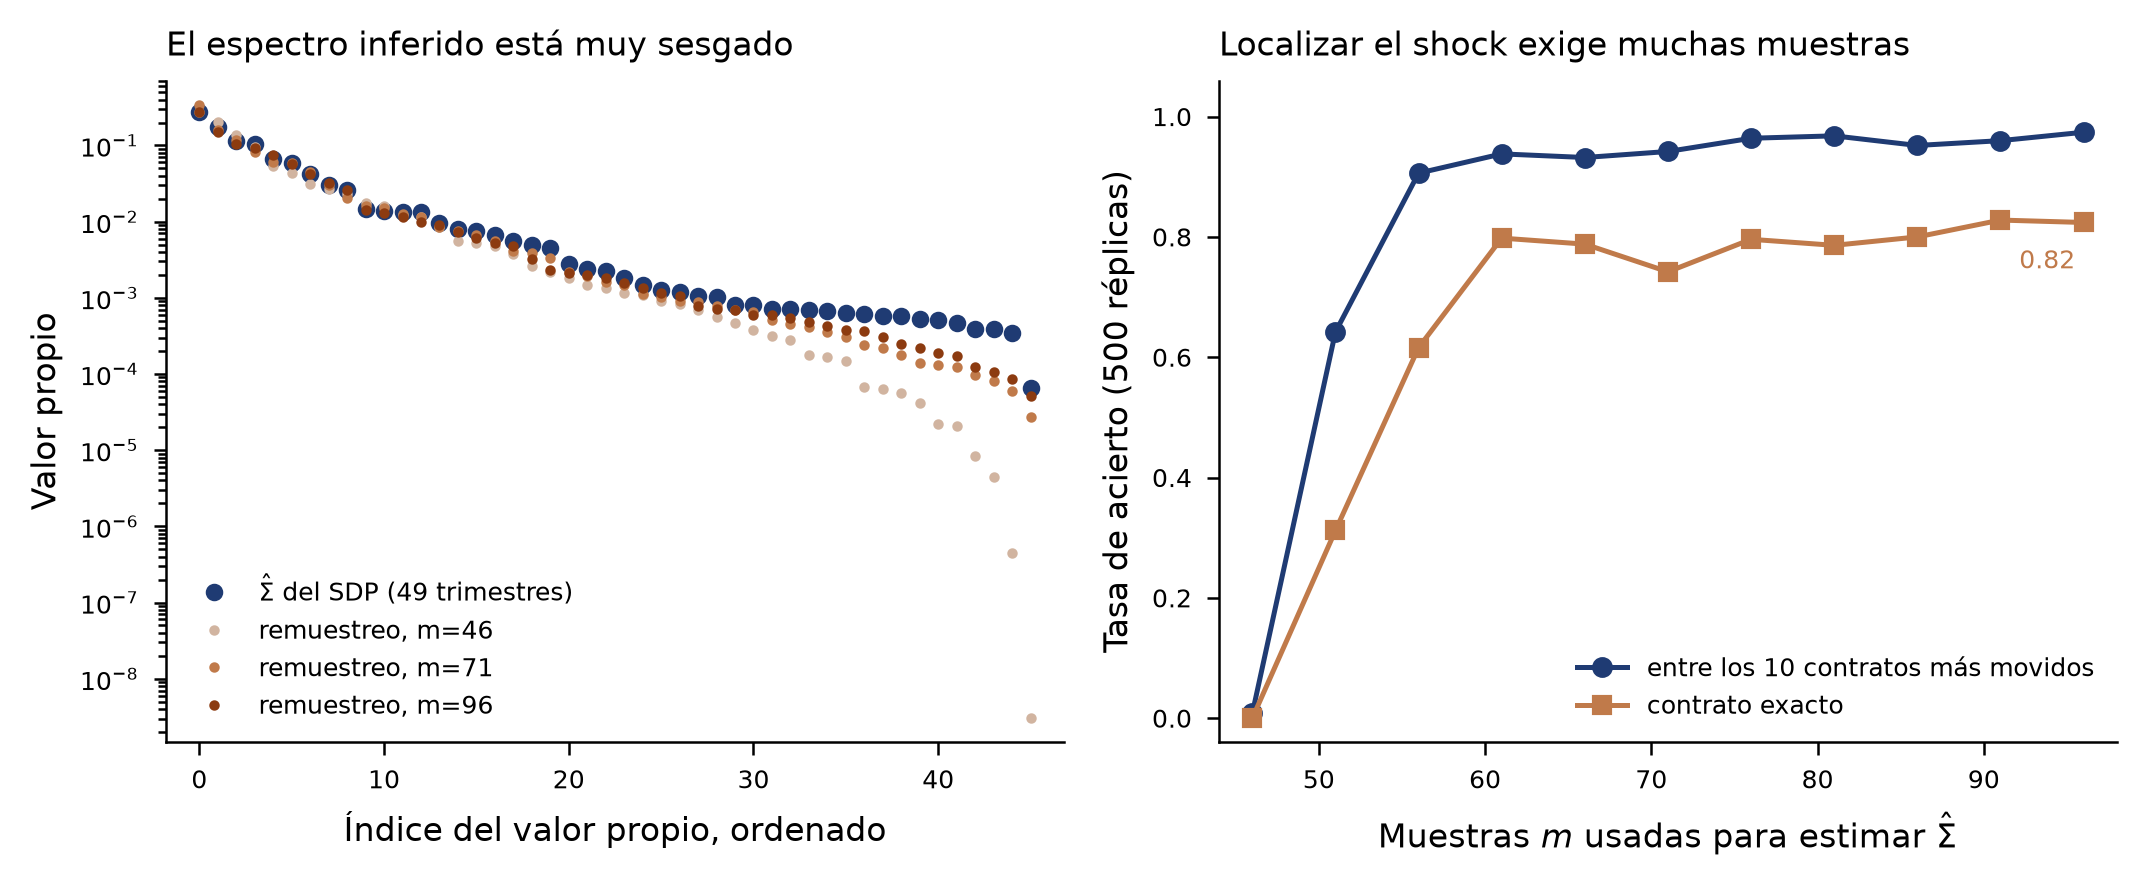
\includegraphics[width=\textwidth]{fig_jalan_ocde_resultados.png}
    \caption[Resultados del caso OCDE reproducidos]{Reproducción de los dos
    resultados empíricos del caso OCDE a partir del repositorio oficial de
    \citeA{jalan_incentive-aware_2024}. El panel izquierdo muestra el espectro de
    la matriz inferida por el programa semidefinido sobre 49 diferencias
    trimestrales, junto con el espectro de estimaciones construidas con $m$
    muestras. El panel derecho muestra la tasa de acierto en el problema de
    detección de la fuente, sobre 500 réplicas por tamaño de muestra.}
    \label{fig:ocde-resultados}
\end{figure}

\section{El levantamiento de datos del caso chileno}
\label{c4:levantamiento}

\subsection{Estrategia de búsqueda y fuentes recorridas}
\label{c4:levantamiento-fuentes}

La diferencia de partida con el caso de referencia es que no existe ningún
repositorio que publique la red del programa como panel. El panel debió
construirse documento a documento, y esa reconstrucción es en sí misma parte del
resultado de este trabajo, porque delimita lo que la información pública permite
afirmar. Se recorrieron cuatro familias de fuentes.

\begin{enumerate}
    \item Cuentas Públicas de CORFO entre 2014 y 2024, revisadas de forma
    íntegra. De ahí se obtuvo el desembolso de CORFO hacia los intermediarios en
    2019, 2020 y 2024, y la colocación de los intermediarios hacia las MiPyMEs en
    2016, 2019, 2020, 2021, 2023 y 2024. La cifra de 2017 corresponde a
    aprobación de líneas por parte del Comité Ejecutivo de Créditos y no a
    desembolso efectivo, el documento principal de 2018 es un escaneo sin capa de
    texto, y la Cuenta Pública de 2022 no reporta ninguna cifra monetaria del
    programa.
    \item Fichas de Monitoreo y Seguimiento de la Oferta Pública de DIPRES entre
    2019 y 2024, junto con el Informe de Detalle de Programas Sociales de cierre
    de 2021. Esta familia entrega la serie más completa del tramo entre CORFO y
    los intermediarios, cubriendo desde 2017 hasta 2024 y además desagregada por
    componente, es decir crédito, leasing y factoring.
    \item Portal estadístico de la Comisión para el Mercado Financiero. La
    revisión confirmó que la CMF no distingue el segmento MiPyME en sus series de
    tasas, ya que la única segmentación disponible es por tramo de monto en
    unidades de fomento, plazo y reajustabilidad. La serie más cercana a lo
    requerido es la estructura de colocaciones comerciales por evaluación de
    riesgo individual y grupal, disponible por banco desde febrero de 2019, que
    sin embargo es saldo de cartera y no flujo de desembolso.
    \item Portal de datos abiertos del Estado. La búsqueda programática con trece
    términos distintos no arrojó ningún conjunto de datos del programa, dado que
    la organización CORFO publica allí solo seis conjuntos, todos de 2012 y 2013 y
    referidos a instrumentos distintos.
\end{enumerate}

Una consecuencia metodológica de este levantamiento es que el estado de cada
celda pasa a ser parte del dato. Cada observación del panel se registra junto con
su fuente, su página y una marca que distingue lo observado de lo faltante, de
modo que el análisis posterior nunca trate como medición lo que en realidad es un
supuesto.

\subsection{El panel obtenido}
\label{c4:levantamiento-panel}

El panel resultante se muestra en la Figura~\ref{fig:panel-comparado}. Antes de
leerlo conviene fijar sobre qué conjunto de aristas se mide la cobertura, porque
no es único. El modelo dual tal como está especificado en la
Sección~\ref{c3:estructura} tiene tres aristas estructurales, que son CORFO con
el intermediario y el intermediario con la MiPyME en la red Tradicional, más el
banco comercial con la MiPyME en la red Alternativa, dado que CORFO y el
intermediario participan solo en la primera y el banco solo en la segunda. A
esas tres se agregan dos aristas que no forman parte de la especificación
original y que el diagnóstico de identificabilidad propone incorporar como
extensión de diseño, que son el fondeo bancario de los propios intermediarios y
las líneas que CORFO coloca a través de bancos comerciales. La grilla de la
figura se construye sobre ese conjunto extendido de cinco aristas, de modo que
las dos últimas filas no deben leerse como datos faltantes de la especificación
vigente sino como la información que haría falta si se adoptara la extensión.

Sobre esa grilla de nueve años hay nueve celdas observadas de cuarenta y cinco.
De las tres aristas estructurales, la que une al banco comercial con la MiPyME
está completamente vacía, mientras que las dos aristas de la red Tradicional
coinciden en 2019, 2020 y 2024, de los cuales solo 2019 y 2020 son años
consecutivos.

\begin{figure}[H]
    \centering
    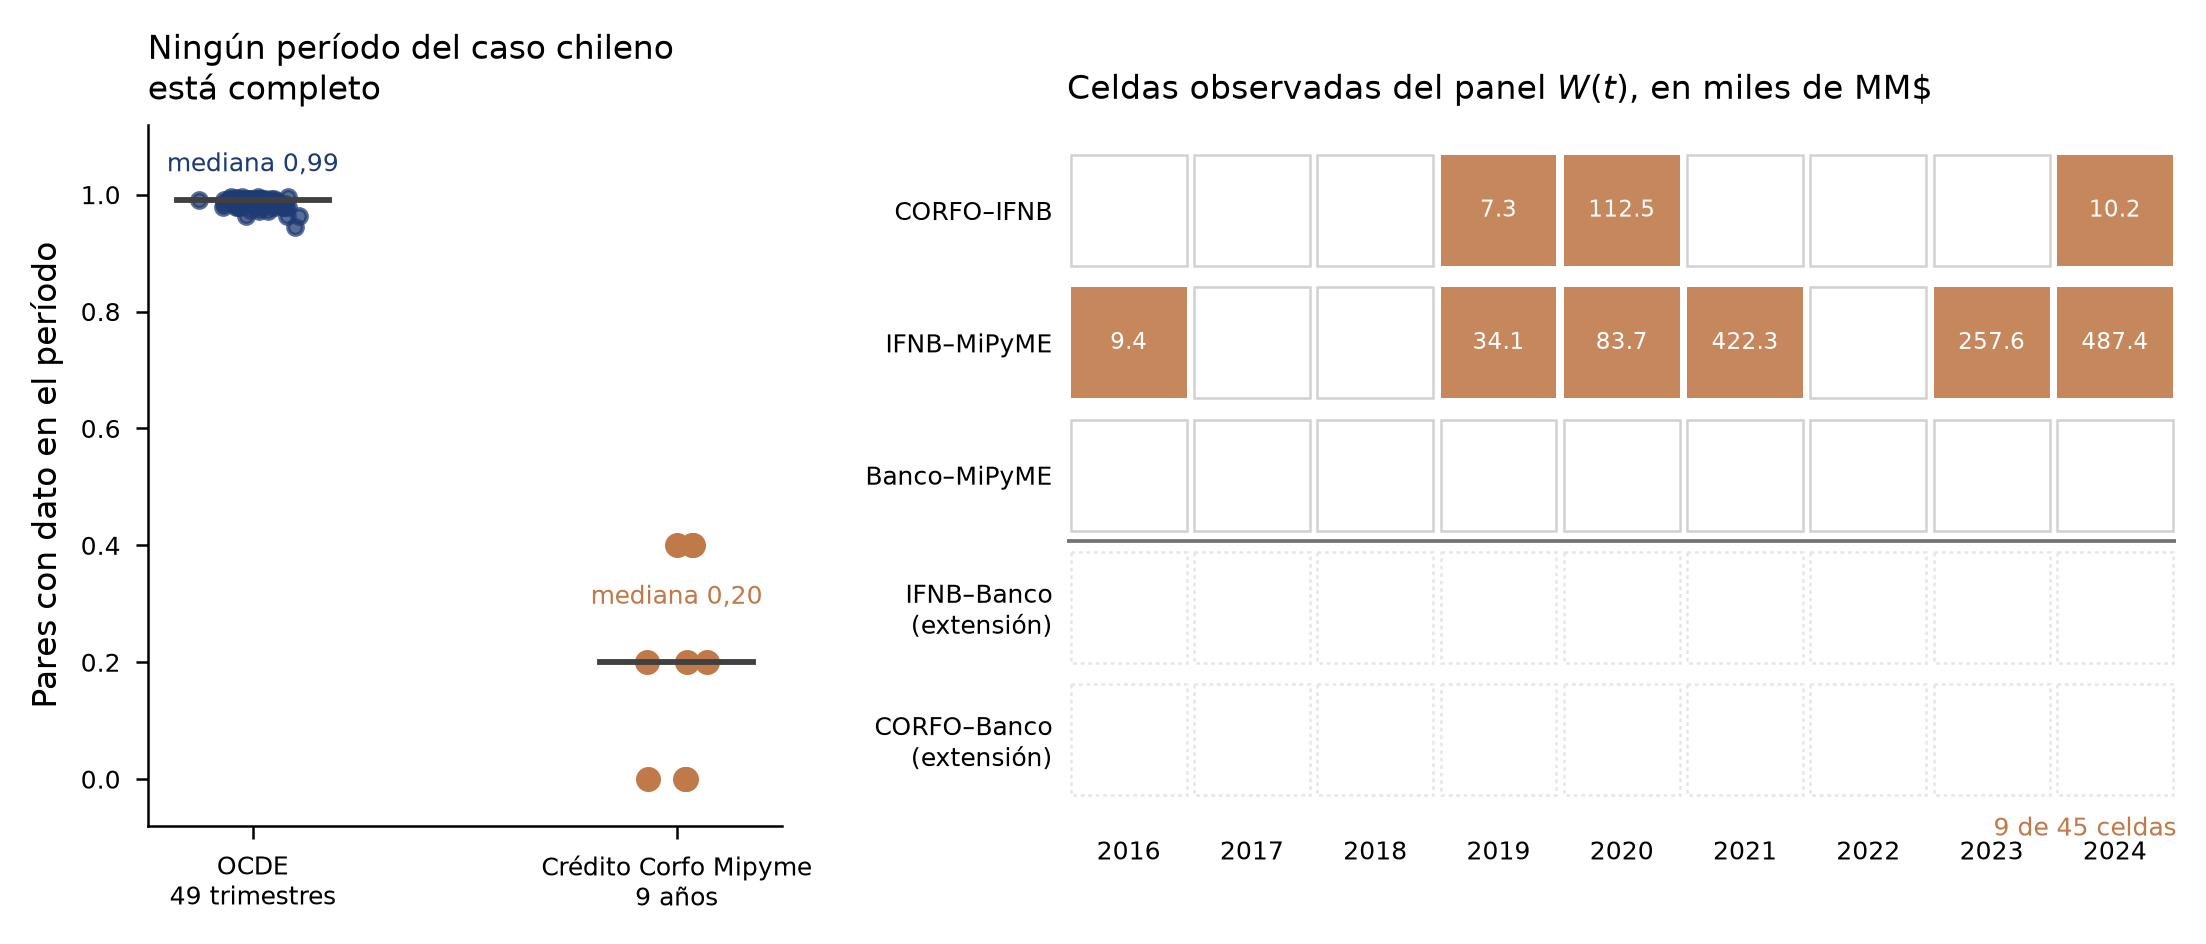
\includegraphics[width=\textwidth]{fig_panel_ocde_vs_corfo.png}
    \caption[Cobertura comparada de ambos paneles]{Cobertura del panel en ambos
    casos. El panel izquierdo compara, período a período, la fracción de pares
    con dato disponible. El panel derecho detalla la grilla del caso chileno, con
    las celdas observadas en miles de millones de pesos y las celdas faltantes en
    blanco. Las dos últimas filas de esa grilla corresponden a la extensión de
    diseño y no a aristas de la especificación vigente del modelo dual.}
    \label{fig:panel-comparado}
\end{figure}

El dato decisivo para el método no es sin embargo el número de celdas, sino el
número de diferencias utilizables, ya que el estimador de la Proposición~1 opera
sobre $W(t+1)-W(t)$ y una sola celda faltante elimina el período completo. Bajo
ese criterio el recuento depende de qué red se considere. Para la red de cuatro
agentes, en cualquiera de sus dos versiones, no hay ninguna diferencia
utilizable, porque ningún año tiene completas todas sus aristas. Restringiendo
la mirada a la red Tradicional por separado, que involucra únicamente a CORFO,
al intermediario y a la MiPyME, hay exactamente una diferencia utilizable, que
es la que va de 2019 a 2020, frente a los seis parámetros libres de la $\Sigma$
de tres agentes. Esa única diferencia tampoco alcanzaría aunque se dispusiera de
muchas más, ya que el rango de la información en esa cadena es de 3 sobre 6,
según se detalla en la Sección~\ref{c4:comparacion}.

\subsection{Obstáculos de comparabilidad detectados}
\label{c4:levantamiento-obstaculos}

Además de la cobertura, el levantamiento dejó al descubierto cuatro problemas que
afectan la comparabilidad de las cifras entre sí.

\begin{enumerate}
    \item Ambigüedad entre flujo y saldo. Las Cuentas Públicas reportan
    desembolsos, mientras que la serie bancaria más cercana de la CMF reporta
    saldos de cartera vigente, y el modelo trata la arista como una posición
    única, por lo que mezclar ambas naturalezas entre aristas rompe la
    comparabilidad.
    \item Multiplicidad de bases de pesos reales. Las fichas de DIPRES reexpresan
    cada año en la base del año de publicación, de modo que un mismo ejercicio
    aparece con cifras distintas según la ficha que se consulte. El gasto de 2018
    figura como 12.517,5 millones de pesos de 2020 y como 12.459,3 millones de
    pesos de 2021, mientras que el de 2019 figura como 7.519,0 y como 7.658,4 en
    esas mismas dos bases.
    \item Períodos parciales. La cifra de 2018 cubre entre enero y noviembre, y
    la de 2021 también, de manera que ninguna de las dos es comparable con un año
    completo sin un ajuste declarado.
    \item Distinción entre aprobación y desembolso. La única cifra disponible
    para 2017 corresponde a líneas de crédito aprobadas y no a montos girados.
\end{enumerate}

A estos cuatro se suma un problema de agregación. Las fuentes públicas reportan a
los intermediarios como un único agregado, de modo que la red observable tiene un
solo nodo intermediario, cuando en realidad el programa opera con varias
instituciones distinguibles entre sí.

\section{Comparación de los dos casos}
\label{c4:comparacion}

La Tabla~\ref{tab:comparacion-ocde-corfo} resume el contraste entre ambos
ejercicios en las dimensiones que el método vuelve relevantes.

\begin{table}[H]
    \centering
    \small
    \caption[Comparación entre el caso OCDE y el caso chileno]{Comparación entre
    el ejercicio empírico de \citeA{jalan_incentive-aware_2024} y el panel
    levantado para el programa Crédito Corfo Mipyme.}
    \label{tab:comparacion-ocde-corfo}
    \begin{tabular}{p{3.2cm}p{4.6cm}p{5.4cm}}
        \toprule
        Dimensión & Caso OCDE & Crédito Corfo Mipyme \\
        \midrule
        Agentes $n$ & 46 & 4 \\
        Pares posibles & 1.035 & 6 \\
        Aristas admisibles & 1.035, solo se prohíbe el lazo propio & 3 estructurales, más 2 en la extensión de diseño \\
        Períodos & 50 trimestres entre 2010 y 2022 & 9 años entre 2016 y 2024 \\
        Diferencias utilizables & 49 & 0 en la red de cuatro agentes y 1 en la red Tradicional sola \\
        Celdas observadas & 50.715 de 50.715 & 9 de 45 en la grilla extendida \\
        Entradas no nulas & 98,50 \% & no evaluable \\
        Parámetros de $\Sigma$ & 1.081 & 10 \\
        Ecuaciones por parámetro & 46,9 & 0 \\
        Rango de la información & 21 de 21 en el análogo completo con $n=6$ & 5 de 10 en la cadena de cuatro agentes y 3 de 6 en la red Tradicional sola \\
        Identificación de $\Sigma$ & sí & no \\
        Peso de la arista & suma de los flujos en ambos sentidos & desembolso en un solo sentido \\
        Medición & flujo comercial en una sola base & mezcla de flujo y saldo en cuatro bases distintas \\
        Obtención & descarga única desde un repositorio estadístico & reconstrucción documento a documento \\
        \bottomrule
    \end{tabular}
\end{table}

De esa comparación se desprenden tres diferencias, y conviene distinguirlas
porque no son todas igualmente reparables.

\paragraph{Diferencia de volumen.} Es la más visible y a la vez la menos grave,
ya que depende únicamente de la periodicidad y de la cobertura de la fuente. La
solicitud de información cursada a CORFO, que pide registros mensuales entre
enero de 2016 y diciembre de 2024, llevaría el panel de nueve observaciones
anuales a 108 períodos y 107 diferencias, con lo que el volumen dejaría de ser la
restricción activa.

\paragraph{Diferencia de topología.} Es la decisiva y no se repara con más datos
del mismo tipo. La red que entregan los registros de CORFO está formada por
CORFO, por los intermediarios y por las MiPyMEs, y es bipartita, puesto que
CORFO y las MiPyMEs quedan de un lado y los intermediarios del otro, sin ninguna
arista dentro de cada lado, mientras que la red de la OCDE es prácticamente
completa. En una red bipartita el residuo del estimador solo toca entradas de
$\Sigma$ dentro de cada lado, de modo que ninguna cantidad de meses ni de
intermediarios adicionales informa sobre el resto.

Esa misma lectura explica por qué la extensión de diseño descrita en la
Sección~\ref{c4:levantamiento-panel} sí repara la identificación, y conviene
distinguir el papel de cada una de sus dos aristas. El fondeo bancario de los
intermediarios une a dos agentes que están del mismo lado, de manera que es la
única de las dos que rompe la bipartición. Las líneas que CORFO coloca a través
de bancos comerciales, en cambio, cruzan de un lado al otro y por lo tanto no la
rompen, aunque el cálculo de rango muestra que de todos modos hacen falta,
puesto que solo con ambas aristas presentes a la vez el rango pasa de 18 a 21
sobre 21. El carácter bipartito de la red del programa es un aporte propio del
presente trabajo y no una consecuencia enunciada en la fuente, dado que los
resultados de identificación de dicho artículo se formulan para redes sin
aristas prohibidas.

\paragraph{Diferencia de homogeneidad de la medición.} El Supuesto~1 exige que la
volatilidad de las creencias sea la misma en todas las aristas. En la red de la
OCDE todas las aristas son comercio entre pares del mismo tipo, mientras que en
el programa el tramo que va de CORFO hacia los intermediarios es administrado,
porque las tasas las fija un comité y la asignación se hace por licitación, y por
lo tanto no es un proceso de creencias de mercado. Este es el supuesto más frágil
del traslado y debe declararse como tal.

\subsection{Una precisión sobre el uso del Teorema 5}
\label{c4:precision-teorema5}

El diagnóstico muestral del Capítulo~\ref{c3} aplica la cota del Teorema~5 al
largo del panel disponible. Corresponde precisar esa lectura, porque el teorema y
el panel se refieren a objetos distintos. La cantidad $m$ que aparece en la
Ecuación~\eqref{eq:teorema5} es el número de muestras de retornos con que cada
agente estima su propia covarianza $\hat\Sigma_i$, y el resultado acota cuánto se
degrada el factor de amortiguación seguro de las negociaciones bilaterales cuando
esa estimación es imperfecta. En cambio el largo del panel $W(t)$ es el insumo de
la ruta alternativa, que es la Proposición~1 de la Ecuación~\eqref{eq:prop1},
donde lo que se estima es una $\Sigma$ común a partir de los incrementos de la
red observada. La propia Sección~\ref{c24:identificacion} presenta ambas rutas
como alternativas entre sí.

La precisión tiene dos consecuencias. La primera es que la cota de seis
observaciones no es el criterio que decide si el panel alcanza, puesto que el
criterio pertinente es cuántas diferencias completas $\Delta W$ existen, y hoy
son cero. La segunda es que el Teorema~5 supone explícitamente que no hay aristas
prohibidas, condición que la red del programa no cumple, de modo que su cota no
es directamente aplicable al caso. El diagnóstico de insuficiencia del panel se
sostiene igualmente, pero su fundamento correcto es la combinación de ausencia de
diferencias utilizables y déficit de rango por bipartición, y no el
incumplimiento de la cota del Teorema~5.

\section{Alcance del análisis con la información disponible}
\label{c4:alcance}

El contraste anterior permite ordenar el trabajo restante en tres niveles, según
de quién dependa cada uno.

\paragraph{Resultados que ya son concluyentes.} No dependen de ninguna entrega
pendiente y corresponden al diagnóstico de identificabilidad, es decir la
bipartición de la red del programa y el déficit de rango que de ella se sigue, la
caracterización de qué entradas de $\Sigma$ serían recuperables y cuáles no, y la
auditoría del estimador publicado junto con la corrección propuesta.

\paragraph{Resultados que se desbloquean con la entrega de CORFO.} Con registros
mensuales e intermediarios distinguidos uno a uno, el panel pasa a 107
diferencias y la red a $1+k+1$ nodos, lo que permite estimar las covarianzas
entre pares de intermediarios y la covarianza entre CORFO y la MiPyME, que son
precisamente las entradas que el cálculo de rango señala como recuperables en una
red bipartita.

\paragraph{Resultados que requieren fuentes externas a CORFO.} La identificación
completa de $\Sigma$ exige dos aristas que deben levantarse simultáneamente, que
son el fondeo bancario de los propios intermediarios, única de las dos que rompe
la bipartición, y las líneas que CORFO coloca a través de bancos comerciales. La
primera no pertenece al ámbito de CORFO y debe buscarse en la información de la
CMF o en los estados financieros de los intermediarios.

Mientras esas entregas no se concreten, el análisis que este capítulo habilita es
de naturaleza comparativa y estructural, en el sentido de que establece qué exige
el método, cuánto de eso cubre la información pública chilena y qué faltaría
exactamente para cerrar la brecha, lo que constituye el punto de partida del
análisis cuantitativo que continúa en las secciones siguientes.

\chapter{Conclusiones y Recomendaciones}
\label{c5} % la etiqueta para referencias





% Ingenieros prefieren la bibliografia antes que los anexos

\cleardoublepage

\addcontentsline{toc}{chapter}{Bibliografía}

\bibliographystyle{newapa}
\bibliography{referencias}

\appendix % seguido de archivos de apendices

\cleardoublepage

% Escribe 'Anexos' en el Indice General
\addcontentsline{toc}{chapter}{Anexos}

% anexo_a.tex

\chapter{Anexos}
\label{anexos}

\section{Notación del modelo}
\label{anexo:notacion}

La Tabla~\ref{tab:notacion} reúne los símbolos empleados en el Capítulo~\ref{c2}
y en el Capítulo~\ref{c3}, con el significado que cada uno tiene en el modelo de
\citeA{jalan_incentive-aware_2024} y en su extensión dual de
\citeA{venegas_dual_network_2024}.

\begin{table}[htbp]
\centering
\caption[Notación del modelo de redes duales]{Notación empleada en el documento para el modelo de redes duales y su calibración empírica.}
\label{tab:notacion}
\small
\begin{tabular}{ll}
\hline
Símbolo & Significado \\
\hline
$W$ & Matriz simétrica de tamaños de contrato. $W_{ij}$ es el contrato vigente entre $i$ y $j$ \\
$P$ & Matriz antisimétrica de precios o pagos laterales entre pares de agentes \\
$M$ & Matriz de creencias de retorno esperado. $\mu_i = Me_i$ es el vector de creencias de $i$ \\
$\Sigma_i$ & Matriz de covarianza de retornos percibida por el agente $i$ \\
$\gamma_i$ & Coeficiente de aversión al riesgo del agente $i$ \\
$\Gamma$ & Matriz diagonal que agrupa los $\gamma_i$ de todos los agentes \\
$\Psi_i$ & Matriz que codifica qué contrapartes tiene permitidas el agente $i$ \\
$Q_i$ & Matriz de sensibilidad del agente $i$, definida en la Ecuación~\eqref{eq:optimo} \\
$F$ & Conjunto de pares $(i,j)$ con $i<j$ donde el precio $P_{ij}$ puede ser no nulo \\
$Z_F$ & Matriz de coeficientes del sistema de precios de la Ecuación~\eqref{eq:teorema1} \\
$\eta$ & Factor de amortiguación del algoritmo de negociación bilateral, Ecuación~\eqref{eq:eta} \\
$\lambda_A$ & Parámetro de fricción de acceso a la red Alternativa (modelo dual) \\
$\tau$ & Parámetro de transparencia o fricción del modelo dual \\
$m$ & Número de observaciones históricas por agente para estimar $\Sigma_i$ \\
$n$ & Número de agentes de la red. En el caso de aplicación, $n=4$ \\
\hline
\end{tabular}
\end{table}

\section{Fuentes de datos consultadas}
\label{anexo:fuentes}

La Tabla~\ref{tab:fuentes} detalla las fuentes revisadas durante el
levantamiento descrito en la Sección~\ref{c3:datos}, el régimen de acceso de
cada una y el insumo que aporta a la calibración del modelo.

\begin{table}[htbp]
\centering
\caption[Fuentes de datos consultadas para la calibración empírica]{Fuentes de datos consultadas, régimen de acceso e insumo que aporta cada una a la calibración del caso CORFO--Intermediario--MiPyME--Banco.}
\label{tab:fuentes}
\small
\begin{tabular}{p{0.26\textwidth}p{0.12\textwidth}p{0.50\textwidth}}
\hline
Fuente & Acceso & Insumo que aporta \\
\hline
Cuentas Públicas Participativas de CORFO, colección 2014--2024 & Público &
Monto de préstamos de CORFO a los IFNB ($W_{12}$) para 2019, 2020 y 2024, y
cifra de colocaciones del programa antecesor Microcrédito para 2016 \\
DIPRES, Informe de Detalle de Programas Sociales, cierre 2021 & Público &
Tasa de interés mayorista CORFO$\to$IFNB, de 4,23\% a 4,73\% anual \\
DIPRES, ficha de Monitoreo 2021 del programa & Público &
Spread de la tasa a cliente final respecto del benchmark de mercado ACHEF/EFA \\
ELE-7, microdatos \texttt{ele7-full.csv} & Público &
Tasa de interés anualizada del crédito de mayor monto aprobado en 2022, por
tamaño de empresa, empleada como aproximación de $M_{34}$ \\
ELE-7, informe oficial de resultados & Público &
Tasa de rechazo condicional a la solicitud de crédito por tamaño de empresa,
empleada como ancla del supuesto sobre $\lambda_A$ \\
Reglamento operativo del programa Crédito Corfo Mipyme, Texto Refundido, punto 19 & Público &
Establece que los intermediarios rinden mensualmente a CORFO la tasa de interés y
el saldo de capital vigente por operación, información que no es pública y que
resolvería directamente el vacío de $W_{23}$ \\
\hline
\end{tabular}
\end{table}

\section{Entradas de $\Sigma$ recuperables por el estimador}
\label{anexo:entradas}

La Tabla~\ref{tab:entradas-sigma} clasifica las entradas de $\Sigma$ según su tipo y si el estimador de la Proposición~1 las determina, para las dos topologías de la red de registros de CORFO que se evaluaron en la Sección~\ref{c3:identificabilidad}. Una entrada se considera determinada cuando ninguna dirección del núcleo del mapa lineal tiene componente en ella.

\begin{table}[htbp]
\centering
\caption[Entradas de Sigma determinadas por el estimador]{Número de entradas de $\Sigma$ por tipo y estado de identificación. Elaboración propia.}
\label{tab:entradas-sigma}
\small
\begin{tabular}{lcccc}
\hline
Tipo de entrada & Cadena ($k=1$) & Determinadas & Tres intermediarios ($k=3$) & Determinadas \\
\hline
Varianzas propias                        & 3 & 0 & 5 & 0 \\
Covarianzas sobre aristas observadas     & 2 & 0 & 6 & 0 \\
Covarianzas entre agentes sin contrato   & 1 & 1 & 4 & 4 \\
\hline
Total                                    & 6 & 1 & 15 & 4 \\
\hline
\end{tabular}
\end{table}

\section{Auditoría del estimador de la Proposición 1}
\label{anexo:auditoria}

Este anexo desarrolla la auditoría numérica del estimador de $\Sigma$ que se
resume en la Sección~\ref{c4:ocde-procedimiento}. El motivo de auditarlo es que
la calibración que este trabajo persigue necesita una estimación puntual de
$\Sigma$, mientras que los dos análisis del artículo de referencia solo
requieren su espectro y una tasa de acierto relativa, de modo que el estimador
nunca fue evaluado para el uso que aquí se le quiere dar.

\subsection{Diseño del experimento}
\label{anexo:auditoria-diseno}

La auditoría evalúa el estimador en la condición más favorable posible, que es
aquella en que los datos provienen exactamente del proceso que el método supone.
Se generan paneles sintéticos bajo el Supuesto~1 del artículo, es decir con
aversión al riesgo unitaria, una matriz de covarianzas constante en el tiempo y
cada entrada de la matriz de creencias evolucionando como un movimiento
browniano independiente. Para cada período se resuelve el punto estable exacto
mediante la condición de estabilidad, lo que entrega la red $W(t)$ que el
estimador recibe como dato.

La red elegida es completa y de cuatro agentes, condición necesaria para que el
ejercicio tenga sentido, puesto que el diagnóstico de identificabilidad de la
Sección~\ref{c3:identificabilidad} muestra que en una red con aristas prohibidas
una parte de $\Sigma$ no es recuperable por ningún estimador y el experimento
confundiría ese límite estructural con un defecto del método. En la red completa
de cuatro agentes el rango de la información iguala los diez grados de libertad
de $\Sigma$, de manera que cualquier error remanente es atribuible al estimador
y no a la topología. La matriz verdadera se construye definida positiva y se
normaliza a traza unitaria, igual que la solución del programa semidefinido, y
el error se mide como la norma de Frobenius de la diferencia entre la matriz
estimada y la verdadera, dividida por la norma de esta última.

\subsection{Resultado}
\label{anexo:auditoria-resultado}

La Tabla~\ref{tab:auditoria-estimador} reporta la mediana del error relativo
sobre cinco semillas para cada largo de panel, tanto para el programa
semidefinido publicado como para el estimador corregido que se describe más
abajo.

\begin{table}[htbp]
\centering
\caption[Error relativo del estimador de Sigma segun el largo del panel]{Error
relativo de la matriz estimada respecto de la verdadera, en función del número de
períodos observados. Mediana sobre cinco semillas, con el rango observado entre
paréntesis. Elaboración propia sobre paneles sintéticos generados bajo el
Supuesto~1 en una red completa de cuatro agentes.}
\label{tab:auditoria-estimador}
\small
\begin{tabular}{rcc}
\hline
Períodos $T$ & Programa semidefinido publicado & Estimador corregido \\
\hline
5   & 0,92 \ (0,75 a 1,21) & 0,62 \ (0,49 a 0,71) \\
20  & 0,71 \ (0,58 a 0,84) & 0,38 \ (0,33 a 0,44) \\
40  & 0,50 \ (0,42 a 0,63) & 0,26 \ (0,21 a 0,35) \\
80  & 0,41 \ (0,34 a 0,50) & 0,16 \ (0,07 a 0,20) \\
160 & 0,39 \ (0,29 a 0,48) & 0,12 \ (0,09 a 0,15) \\
\hline
\end{tabular}
\end{table}

El patrón distingue con claridad los dos comportamientos. El estimador publicado
desciende mientras el panel es corto y luego se detiene alrededor de $0{,}39$,
sin que duplicar el número de períodos de 80 a 160 produzca una mejora
apreciable. El estimador corregido, en cambio, sigue descendiendo en todo el
rango explorado y llega a $0{,}12$, comportamiento propio de un estimador que
converge.

\subsection{Por qué se trata de un sesgo del criterio}
\label{anexo:auditoria-causa}

Un estancamiento del error admite dos explicaciones, a saber, que el
solucionador numérico no alcance el mínimo del problema o que el mínimo del
problema no esté en la matriz verdadera. Ambas se distinguen evaluando la propia
función objetivo del programa semidefinido en las dos matrices. Con un panel de
160 períodos, el objetivo vale $871{,}13$ en la matriz estimada y $939{,}02$ en
la verdadera. Como la matriz estimada alcanza un valor estrictamente menor, el
solucionador no está fallando, sino resolviendo correctamente un problema cuyo
óptimo no coincide con la respuesta buscada. El defecto está, por lo tanto, en
el criterio y no en su implementación.

El origen del problema se localiza en la derivación del Apéndice A.11 del
artículo, que llega al programa semidefinido en dos pasos. El primero establece
que, bajo el Supuesto~1, la trayectoria de creencias más probable dadas las
redes observadas es la que minimiza la suma de los cambios cuadráticos
$\sum_t \|M(t+1)-M(t)\|_F^2$, resultado que se obtiene maximizando la densidad
posterior de $M(1),\dots,M(T)$ condicional en $W(1),\dots,W(T)$ y en $\Sigma$. En
esa posterior, el factor que vincula las redes con las creencias aparece como
función indicadora de la condición de punto estable, es decir, vale uno cuando la
condición se cumple y cero en caso contrario. El segundo paso despeja
$M(t)+M(t)^\top$ en función de $W(t)$ y de $\Sigma$ mediante esa misma condición
y lo sustituye en el objetivo, con lo que se obtiene un programa expresado en
$\Sigma$.

La dificultad está en que el criterio así obtenido es el que selecciona la
trayectoria de creencias más probable para una $\Sigma$ dada, y no la $\Sigma$
más probable dadas las redes. Convertir el primero en el segundo exige el cambio
de variable que lleva de $M$ a $W$, cuyo jacobiano depende de $\Sigma$, puesto
que la relación entre ambas es lineal con matriz $\Sigma\otimes I + I\otimes\Sigma$.
Ese factor no aparece en la derivación. Su omisión no es inocua, dado que el
objetivo publicado puede reducirse encogiendo $\Sigma$ en las direcciones que
más pesan en el residuo, y la restricción de traza unitaria no lo impide porque
fija únicamente la escala global y no la forma de la matriz. De ahí que la
estimación resulte sistemáticamente contraída hacia esas direcciones.

\subsection{El estimador corregido}
\label{anexo:auditoria-correccion}

La corrección consiste en reponer el término omitido. Denotando por
$B_\Sigma$ la matriz del mapa lineal que lleva las diferencias de red a los
residuos sobre los pares permitidos, y por $Q(\Sigma)=\sum_t \|B_\Sigma\,
\Delta W(t)\|^2$ el residuo acumulado, la verosimilitud perfilada conduce a
minimizar
\begin{equation}
\label{eq:mle-corregido}
    \frac{|F|}{2}\,\log Q(\Sigma) \;-\; \log\left|\det B_\Sigma\right| ,
\end{equation}
donde $|F|$ es el número de pares permitidos. El primer término reproduce el
criterio publicado en escala logarítmica y el segundo es el jacobiano ausente.
El objetivo de la Ecuación~\eqref{eq:mle-corregido} resulta invariante a la
escala de $\Sigma$, de modo que la normalización de traza unitaria deja de
cumplir un papel sustantivo y pasa a ser una convención de presentación. Los
valores de la columna derecha de la Tabla~\ref{tab:auditoria-estimador}
corresponden a minimizar esta expresión.

\subsection{Alcance del hallazgo}
\label{anexo:auditoria-alcance}

Esta auditoría no invalida ningún resultado del artículo de referencia. Los dos
análisis que sus autores construyen sobre la matriz estimada, que son el estudio
de su espectro y el problema de detección de la fuente de un cambio en las
creencias, dependen de propiedades relativas y no de su exactitud puntual, por
lo que un sesgo de contracción no los compromete. La corrección es necesaria
únicamente para el uso que este trabajo le da al estimador, que es obtener una
$\Sigma$ con la cual calcular niveles de bienestar y contrafactuales, donde la
diferencia entre un error de $0{,}39$ y uno de $0{,}12$ sí incide en las
magnitudes que se reportan.

\section{Diagnóstico de la especificación dual}
\label{anexo:dual}

Este anexo desarrolla los tres puntos que la Sección~\ref{c4:venegas-dual}
resume, a saber la tensión entre las dos contabilidades del riesgo, la brecha
que produce fragmentar una exposición en dos redes y la incompatibilidad del
supuesto de precio único con la presencia de una arista prohibida. Todos se
obtuvieron al implementar la capa de acoplamiento que la tesis de
\citeA{venegas_dual_network_2024} no acompaña con código.

\subsection{Las dos contabilidades del riesgo}
\label{anexo:dual-contabilidades}

En el modelo dual cada agente reparte un portafolio total $w_i^{*}$, dado de
antemano, entre la red Tradicional y la Alternativa, de manera que
$w_i^{*} = w_i^{T} + w_i^{A}$. La pregunta que decide todo lo demás es sobre qué
objeto se evalúa el término de riesgo de la utilidad.

Si el riesgo se evalúa por separado en cada red, la utilidad del agente incluye
los dos términos $w_i^{T\top}\Sigma_i w_i^{T}$ y $w_i^{A\top}\Sigma_i w_i^{A}$.
En ese caso el problema del agente es estrictamente cóncavo en $w_i^{T}$, su
Hessiano es $H_i = 2\gamma_i\Sigma_i + \lambda_A I$ y existe un óptimo interior,
que con transparencia y fricción nulas entrega $w_i^{T} = \tfrac{1}{2}w_i^{*}$,
es decir el reparto por mitades que la fuente publica.

Si en cambio el riesgo se evalúa sobre la exposición combinada, el término
cuadrático es $w_i^{*\top}\Sigma_i w_i^{*}$, que no depende del reparto porque
$w_i^{*}$ está fijo por supuesto. El Hessiano colapsa entonces a
$H_i = \lambda_A I$, sin intervención de $\Sigma_i$, y con $\lambda_A = 0$, que
es el valor declarado para los escenarios de validación, el problema pasa a ser
lineal en $w_i^{T}$. Un problema lineal sin cotas no tiene óptimo interior, de
modo que el agente resulta indiferente entre todos los repartos y la cifra de
adopción deja de estar determinada por el modelo.

La dificultad es que la primera contabilidad no reproduce el bienestar publicado
y la segunda sí. Bajo riesgo separado el bienestar total del escenario simétrico
asciende a $2,1507$ y cae a $1,7869$ al activarse la restricción, mientras que
bajo riesgo combinado vale $1,4339$ en ambos casos, que es la cifra que la fuente
reporta. Por lo tanto el reparto por mitades proviene de una contabilidad y la
igualdad del bienestar con la referencia de red única proviene de la otra, sin
que ninguna de las dos produzca ambos resultados.

\subsection{La brecha de fragmentación}
\label{anexo:dual-brecha}

La diferencia entre ambas contabilidades admite forma cerrada. Escribiendo el
reparto como $w_i^{T} = f\,w_i^{*}$ con $f\in[0,1]$, de modo que
$w_i^{A} = (1-f)\,w_i^{*}$, la diferencia entre evaluar el riesgo por separado y
evaluarlo sobre la exposición combinada es
\begin{equation}
\label{eq:brecha-fragmentacion}
    \text{brecha}(f) = 2f(1-f)\sum_i \gamma_i\, w_i^{*\top}\Sigma_i\, w_i^{*}.
\end{equation}
La derivada de la Ecuación~\eqref{eq:brecha-fragmentacion} respecto de $f$ se
anula únicamente en $f = \tfrac{1}{2}$, que es un máximo, de manera que la
sobreestimación crece de forma monótona a medida que el reparto se empareja y
alcanza su valor mayor exactamente en el reparto que la condición de primer orden
elige cuando la transparencia y la fricción son nulas. En el escenario simétrico
de tres agentes la expresión entrega $0,7169$, cifra que coincide con la
diferencia observada entre $2,1507$ y $1,4339$.

La lectura económica de la Ecuación~\eqref{eq:brecha-fragmentacion} es directa.
Al partir una exposición en dos y cobrarle riesgo a cada parte por separado se
omite el término cruzado, que es el que recoge que ambas partes están expuestas
al mismo riesgo subyacente. Esa omisión aparece como una ganancia de bienestar
que no proviene de ninguna mejora en la asignación sino de la mera división del
portafolio.

\subsection{El supuesto de precio único bajo restricción}
\label{anexo:dual-precio}

La definición de asignación factible del modelo dual exige que una misma arista
tenga el mismo precio en ambas redes. Bajo ese supuesto el término lineal del
problema del agente deja de depender del precio, de modo que cada agente resuelve
su reparto de forma aislada y no queda instrumento alguno con el cual conciliar
las dos puntas de una arista.

Sin restricción eso es inocuo, porque el reparto hereda la simetría del
portafolio total. Con la restricción activa en la red Tradicional, en cambio, la
matriz de acceso $\Psi_i$ es distinta para cada agente y el resultado deja de ser
simétrico. La Tabla~\ref{tab:dual-simetria} recoge la asimetría máxima de la
matriz de contratos de la red Tradicional en ambos casos, medida contra la
tolerancia de convergencia del propio motor, que es de $7{,}72\times10^{-4}$ y se
obtiene sobre el portafolio total.

\begin{table}[htbp]
    \centering
    \small
    \caption[Simetría de la red Tradicional bajo precio único]{Asimetría máxima
    de la matriz de contratos de la red Tradicional, según se permita o no que el
    precio difiera entre redes. El punto estable del modelo exige que ambas partes
    acuerden la misma cantidad, de modo que una asimetría muy superior a la
    tolerancia numérica indica que la asignación no es factible. Elaboración
    propia.}
    \label{tab:dual-simetria}
    \begin{tabular}{lcc}
        \toprule
        Escenario & Precio único & Precio distinto por red \\
        \midrule
        Sin restricción & $3{,}86\times10^{-4}$ & $3{,}86\times10^{-4}$ \\
        Con restricción en la red Tradicional & $2{,}27\times10^{-1}$ & $2{,}45\times10^{-4}$ \\
        \bottomrule
    \end{tabular}
\end{table}

La asimetría bajo precio único es dos órdenes de magnitud mayor que la tolerancia,
y se traduce en que una misma arista recibe dos cantidades distintas según desde
qué extremo se la observe. Permitir que el precio difiera entre redes la devuelve
al nivel del ruido numérico, lo que identifica al diferencial de precio entre
redes como el único instrumento que restaura la factibilidad.

\subsection{Un error de transcripción sin consecuencia numérica}
\label{anexo:dual-transcripcion}

Corresponde dejar constancia de un punto menor, detectado al verificar las
derivaciones. La expresión que la tesis imprime para la matriz que resuelve el
problema restringido no satisface la condición de estacionariedad proyectada y,
al evaluarla en el caso sin restricciones, contradice la simplificación que el
propio enunciado declara dos líneas después. La forma que sí resuelve el problema
es análoga a la del artículo base. El punto no afecta ninguna cifra, puesto que
la implementación publicada emplea la forma correcta, de modo que se trata de un
error de redacción y no de cálculo.
    % archivo de apendice

%\input{apendice_b}    % otro archivo de apendice

\label{end}
\end{document}

%%%%%%%%%%%%%%%%%%%%%%%%%%%%%%%%%%%%%%%%%%%%%%%%%%%%%%%%%%%%
